% 第四章 基于DispNetC的立体匹配

\chapter{基于DispNetC的立体匹配}

在双目摄像机拍摄某一场景得到的成对图像中,除去部分由于视角差异导致的遮挡区域,两图的公共视野范围内的像素点应该是一一匹配的,每对匹配点是三维空间中同一个点的投影。立体匹配就是在左右图像中寻找这些匹配点,为它们建立一对一的对应关系的过程。立体匹配结束会得到一张视差图,一般使用灰度图,视差图中的每个点的像素值代表参考图像中对应像素点与其目标图像中的匹配点的视差。真实场景中相邻的像素点经常具有相近的颜色,因此为了获得正确的匹配,就必须找到有效的相似度度量的策略;另外,实际场景中,纹理缺失、纹理重复、遮挡、镜面反射、光照强度差异等问题也给立体匹配带来了很大的困难和挑战。

\begin{figure}[!htb]
	\centering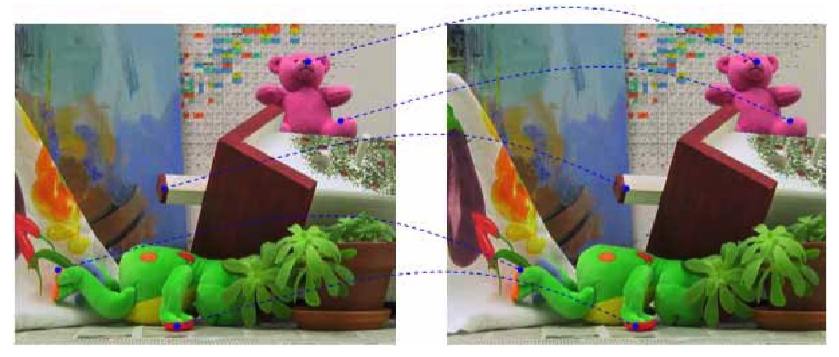
\includegraphics[width=5in]{figures/4_0_stereo_correspondence}
	\caption{立体匹配示意图}\label{fig:4_0_stereo_correspondence}
\end{figure}

% ref: FlowNet paper ch2, Convolutional Networks part.
2012年Krizhevsky等人的工作\cite{krizhevsky2012imagenet}展示了卷积神经网络在大规模图像分类中的良好效果,带动了应用CNN到各种计算机视觉任务中的研究工作。深度卷积神经网络较传统神经网络而言,能够学习到更为复杂的非线性关系,因此能够更好地从大量数据中提取规律。同时其通过卷积操作获得的特征也比人工设计的特征更为有效。

过去几年涌现出了大量使用CNN进行立体匹配的研究成果。KITTI\cite{Menze_2015_CVPR} Stereo Evaluation排行榜的前列已被基于卷积神经网络的算法占领,此类算法在匹配精度和运行时间方面较传统方法都展现出了很明显的优势。Fisher等人\cite{fischer2014descriptor}从通过有监督/无监督训练得到的CNN中提取特征表达,并基于欧氏距离对这些特征进行匹配。Zbontar和LeCun\cite{zbontar2016stereo}训练了一个连体(Siamese)架构的CNN,用来预测图像块之间的相似度。这类基于图像块(patch)的算法的缺点是计算量较大,无法利用全局信息,在计算完匹配代价后仍然需要进行后处理操作,因此并不能显著降低算法的运行时间。

DispNet\cite{mayer2016large}是一种网络结构较为简单、端到端(end-to-end)的立体匹配网络。该网络的运行速度很快,适合应用于无人机等对实时性有较高要求的场景。本章首先简要梳理传统立体匹配算法,然后介绍DispNet的网络结构、训练过程,并给出使用其进行立体匹配的结果。


%------------------------------------------------------------------------------------
\section{传统立体匹配算法简介}
% ref: Robust and real-time stereo matching on parallel graphics hardware...[phd], ch3.2, p83;
% 陈拓ch2.4, p29; 苏东ch2.2.2, p25.
Scharstein\cite{Scharstein2002}对立体匹配领域做了详细的综述,将传统的立体匹配算法分为三类:通过限制搜索像素范围来找到局部最优视差的局部算法;通过定义全局能量函数来得到平滑视差图的全局算法;以及混合了局部与全局算法思想,或不能归类为局部或全局方法的其他算法。

\subsection{全局立体匹配算法}
全局立体匹配算法基于一个能量最小化框架,其寻找使全局能量函数$E(D)$达到最小的视差D:
%
\begin{equation}\label{eq:4_0_energy_function}
E(D) = E_{data}(D) + \lambda E_s(D)
\end{equation}
其中,数据项$E_{data}(D)$描述匹配的代价,平滑项$E_s(D)$显式地引入了对视差变化的平滑约束。$\lambda$是用于平衡数据项和平滑项的比例系数。数据项是整个图像内匹配代价的累计,一般定义为整个匹配集合内每个像素的基于某种差异度量的代价之和:
%
\begin{equation}\label{eq:4_0_energy_function_data_term}
D_{data}(D) = \sum_{p} C(\mathbf{p}, D(\mathbf{p}))
\end{equation}
式中,$C(\mathbf{p}, D(\mathbf{p}))$代表任意一种像素差异度量,用于计算参考图像中点$\mathbf{p} = (x,y)$与目标图像中的匹配点$(x-D(\mathbf{p}),y)$之间的代价。常用的差异性度量有以下几种:

绝对差值和:
\[ SAD(x,y,d) = \sum_{(i,j) \in N} |I_r(x+i, y+j) - I_o(x+i-d, y+j)|  \]

截断绝对差值和:
\[ STAD(x,y,d) = \sum_{(i,j) \in N} min \{ |I_r(x+i, y+j) - I_o(x+i-d, y+j)|  , T \} \]

差值平方和:
\[ SSD(x,y,d) = \sum_{(i,j) \in N} |I_r(x+i, y+j) - I_o(x+i-d, y+j)|^2  \]

归一化互相关:
\[ NCC(x,y,d) = \frac{\sum_{(i,j)\in N} I_r(x+i, y+j)  I_o(x+i-d, y+j) }
{\sqrt   {\sum_{(i,j) \in N} I_r^2(x+i,y+j)  \sum_ {(i,j) \in N} I_o^2(x+i-d, y+j) } }  \]

Census:
\[  Census = \sum_ {(i,j) \in N} HAMMING(I_r(x+i,y+j), I_o(x+i-d, y+j))   \]
式中$I_r$和$I_o$分别表示参考图像和目标图像中的像素灰度值,$N$为窗口范围。前三种匹配代价的时间复杂度为$O(w\times h \times N)$,可以利用积分图像(Integral Image)或箱式滤波(Box Filtering)等方法将时间复杂度降为$O(w \times h)$。

平滑项$E_s(D)$起到正则化的作用,作为惩罚函数来限制局部范围内出现大的视差变动。出于计算方面的考虑,惩罚函数的范围一般被限制在像素点四个直接相邻的邻域$N_4(\mathbf{p})$内,对于点$\mathbf{p}=(x,y)$,$N_4(\mathbf{p}) = \{ (x \pm 1, y), (x, y \pm 1) \}$。 类似于数据项的代价积累,平滑项惩罚并积累相邻像素的视差变化:
\[  E_s(D) = \sum_{\mathbf{p}} \sum_{\mathbf{q} \in N_4(\mathbf{p})} s(\mathbf{p}, \mathbf{q})    \]
$s(\mathbf{p}, \mathbf{q})$表示对相邻像素点$\mathbf{p}$和$\mathbf{q}$的惩罚。

最小化式\ref{eq:4_0_energy_function}中的能量函数被证明为NP困难问题\cite{boykov2001fast},不存在多项式时间内求得最优解的算法,因此一般使用近似算法来寻找最优解附近的次优解。近似算法包括图割\cite{boykov2001fast}、置信传播\cite{sun2003stereo}、动态规划\cite{VanMeerbergen2002}等等。

\subsection{局部立体匹配算法}
局部立体匹配算法是基于窗口的方法,其不使用最小化全局能量函数的框架,而是采用一种称为“赢者通吃”(Winner Takes All)的视差选择策略。对于像素点$\mathbf{p}$,局部算法会遍历设置好的视差搜索范围,取损失最小的视差作为最终的匹配:
%
\begin{equation} \label{eq:4_0_local_WTA}
D(\mathbf{p}) = \arg \min_d C(\mathbf{p}, d)
\end{equation}
注意到上式中并未加入任何平滑约束。基于像素的代价计算会导致获得的视差图中带有很多噪声,并且不能正确匹配有歧义的像素点。为了获得更加可靠的代价,局部立体匹配算法通常会在计算视差前对代价进行累计,累计后的代价是相邻像素代价的加权和。代价累计可以视为一种滤波器:
%
\begin{equation} \label{eq:4_0_local_cost_aggregation}
C(\mathbf{p}, d)' = W(\mathbf{p}) * C(\mathbf{p}, d)
\end{equation}
$C(\mathbf{p}, d)' $是累计后的代价,$C(\mathbf{p}, d)$是各像素的代价,$W(\mathbf{p})$表示点$\mathbf{p}$的“支持窗口”,即一个包含滤波器系数的任意形状和尺寸的窗口。类似于全局方法中的平滑项,代价聚合使得局部方法也能够在匹配过程中加入对平滑的考虑。

最简单的代价聚集使用固定大小和形状的窗口,通常使用一个矩形,并假设窗口内的所有像素点具有相同的视差。这个假设是基于视差平滑约束做出的,但窗口尺寸与代价的聚集之间存在矛盾:窗口尺寸太小,则代价聚集作用不明显,鲁棒性差;而窗口尺寸如果太大,在视差不连续处,窗口内像素点视差相同的假设是不成立的,因此也无法获得较好的结果。因而固定窗口的代价聚集精度不高,但计算比较容易,实时性较好。OpenCV中提供了这种方法的实现,称为块匹配算法(block matching)。

支持窗口可在不同像素点处取不同的尺寸、形状和权重,而这些参数的选择对于保存视差图中的边缘信息非常重要。Veksler\cite{veksler2003fast}提出了自适应窗口尺寸的算法,其使用积分图像的方法从一系列包含感兴趣像素点的不同尺寸的方形窗口中选取最佳的窗口,该方法能够显著地改善获得的视差图的局部平滑性,但其在视差不连续处的精度仍十分有限。Yoon和Kweon\cite{yoon2005locally}提出了自适应支持窗口权重的算法,这种方法极大地提高了局部算法在物体边界处的视差精度,获得了可与部分全局算法相比的匹配效果。

基于十字形(Cross-based)的代价聚合算法\cite{zhang2009cross}是一种自适应窗口形状和尺寸的方法,该方法既利用了感兴趣像素点与其邻域内像素点的像素距离,也利用了它们之间的像素值差异,生成的支持窗口形状并不规则,实时性较好,得到了比较多的应用。
% 陈拓p30还有两段基于双边滤波和基于分割的代价聚合算法。
% <Robust and real-time stereo matching on parallel graphics hardware using gradient-based disparity refinement> p93, 3.2.3 other approaches讲到SGM,陈拓p29全局算法也讲到SGM。按说实验与SGM做了比较,应该介绍一下。。
% TODO: 如果绪论不够,这篇英文博士论文可以抄一抄。
\subsection{其他立体匹配算法}
还有一些立体匹配方法将全局方法与局部方法的思想结合起来,使用非局部的代价聚合策略来扩展基于“赢者通吃”策略的匹配算法,在获得较好的匹配效果的同时,保持了相对较低的计算复杂度。这类算法中最著名的是半全局匹配算法(SGM)\cite{Hirschmuller08}。SGM使用了基于动态规划的代价聚合策略,在16个方向上使用一维动态规划进行代价累计然后求和,从而得到近似二维优化的效果。该算法在现实中得到了广泛的应用。


%------------------------------------------------------------------------------------
% TODO: 立体匹配步骤这一小节要不要?
%\subsection{立体匹配步骤}
%% ref: 陈拓ch2.2.3, p26.
%Scharstein\cite{Scharstein2002}通过对各种立体匹配算法进行研究,将传统立体匹配算法归为以下四个步骤:
%
%(1)匹配代价计算




%------------------------------------------------------------------------------------
\section{DispNet网络结构}
% ref: FlowNet paper ch3; DispNet paper ch5.
DispNet是一种端到端的立体匹配卷积神经网络模型。所谓“端到端”是指输入需要匹配的左右图,即可预测得到匹配结果,无需其他后处理操作。其借鉴了用于预测光流的FlowNet\cite{dosovitskiy2015flownet}的结构并将其应用于立体匹配领域。

在卷积神经网络中,池化对于降低训练网络的训练量是必要的,而且能够使得网络具备聚合输入图像中更大范围信息的能力。但是池化会导致分辨率下降,为了获得稠密的与输入图像具有相同分辨率的预测结果,我们需要对池化后得到的粗糙结果进行细化。因此DispNet网络的结构呈沙漏形(如图\ref{fig:4_1_dispnet_shape}),包含一个收缩部分和一个扩张部分,整个网络作为一个整体,使用反向传播算法来训练。

\begin{figure}[!htb]
	\centering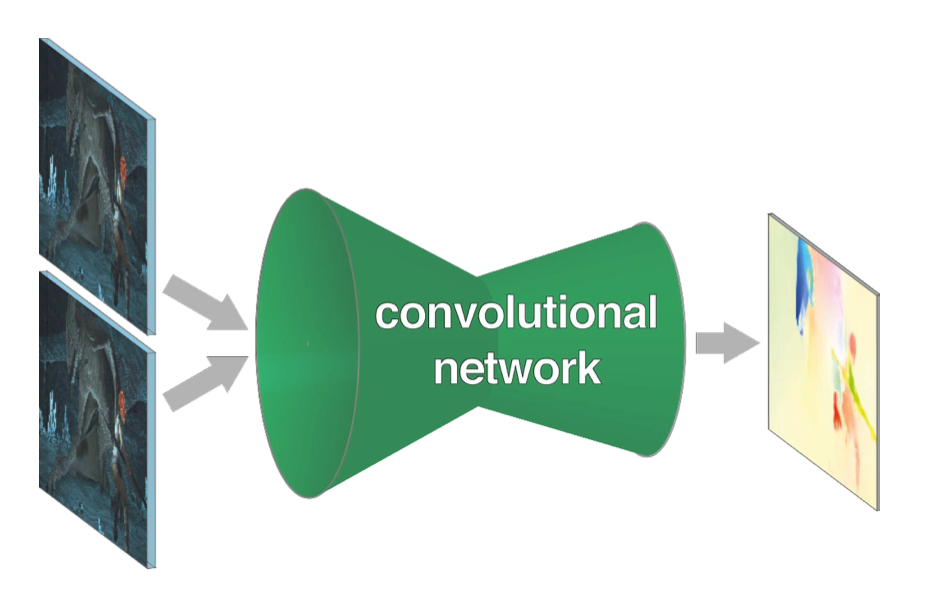
\includegraphics[width=3.5in]{figures/4_1_dispnet_shape.png}
	\caption{沙漏型的网络结构\cite{dosovitskiy2015flownet}}\label{fig:4_1_dispnet_shape}
\end{figure}

\subsubsection{收缩部分}
DispNet的收缩部分包括10个卷积层,其中前两个卷积层的卷积核尺寸分别为$7\times 7$和$5\times 5$,其余卷积层的卷积核尺寸为$3\times 3$。10个卷积层中有6个取步长为2,其余为1,故一共进行了64倍的下采样。

网络的输入为一对图片,最简单的处理方式是将两张图片直接堆叠在一起输入网络,让网络自己学习如何处理成对的图像来获取所需的深度信息。每张图片有RGB三个通道,故网络输入的厚度为6。这种只包含卷积层的网络架构是DispNet的基础架构,如图\ref{fig:4_1_DispNet}所示。图中标注的数字为“分辨率@通道数(特征图层数)”。

\begin{figure}[!htbp]
	\centering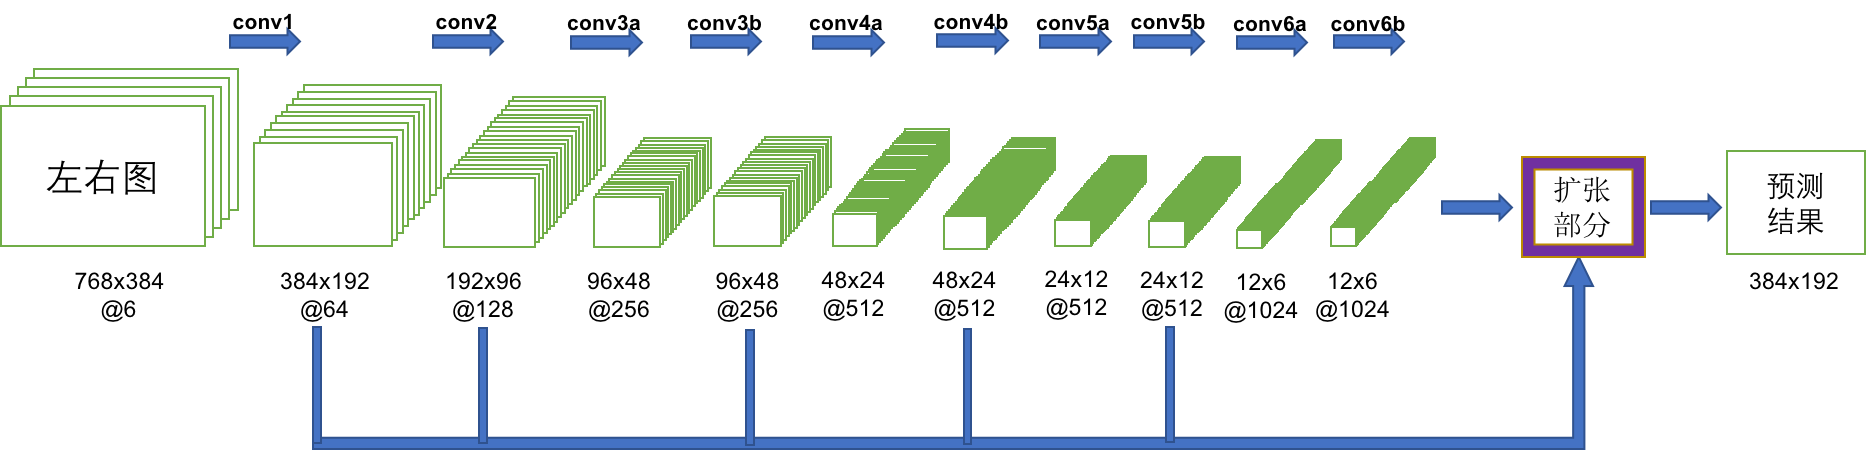
\includegraphics[width=6in]{figures/4_1_dispnet_architecture}
	\caption{DispNet网络基础架构}\label{fig:4_1_DispNet}
\end{figure}

另一种处理方式是建立两个相互独立但相同的结构来分别处理输入的左右图,之后通过一定方式将它们组合起来,如图\ref{fig:4_1_DispNetC}所示。网络首先分别从两张图片生成一些有价值的特征表达,然后在更高级别将它们联系起来。这种结构有些类似于传统的匹配模式:首先从两张图片的小块区域中提取特征,然后比较获得的特征向量。

\begin{figure}[!htb]
	\centering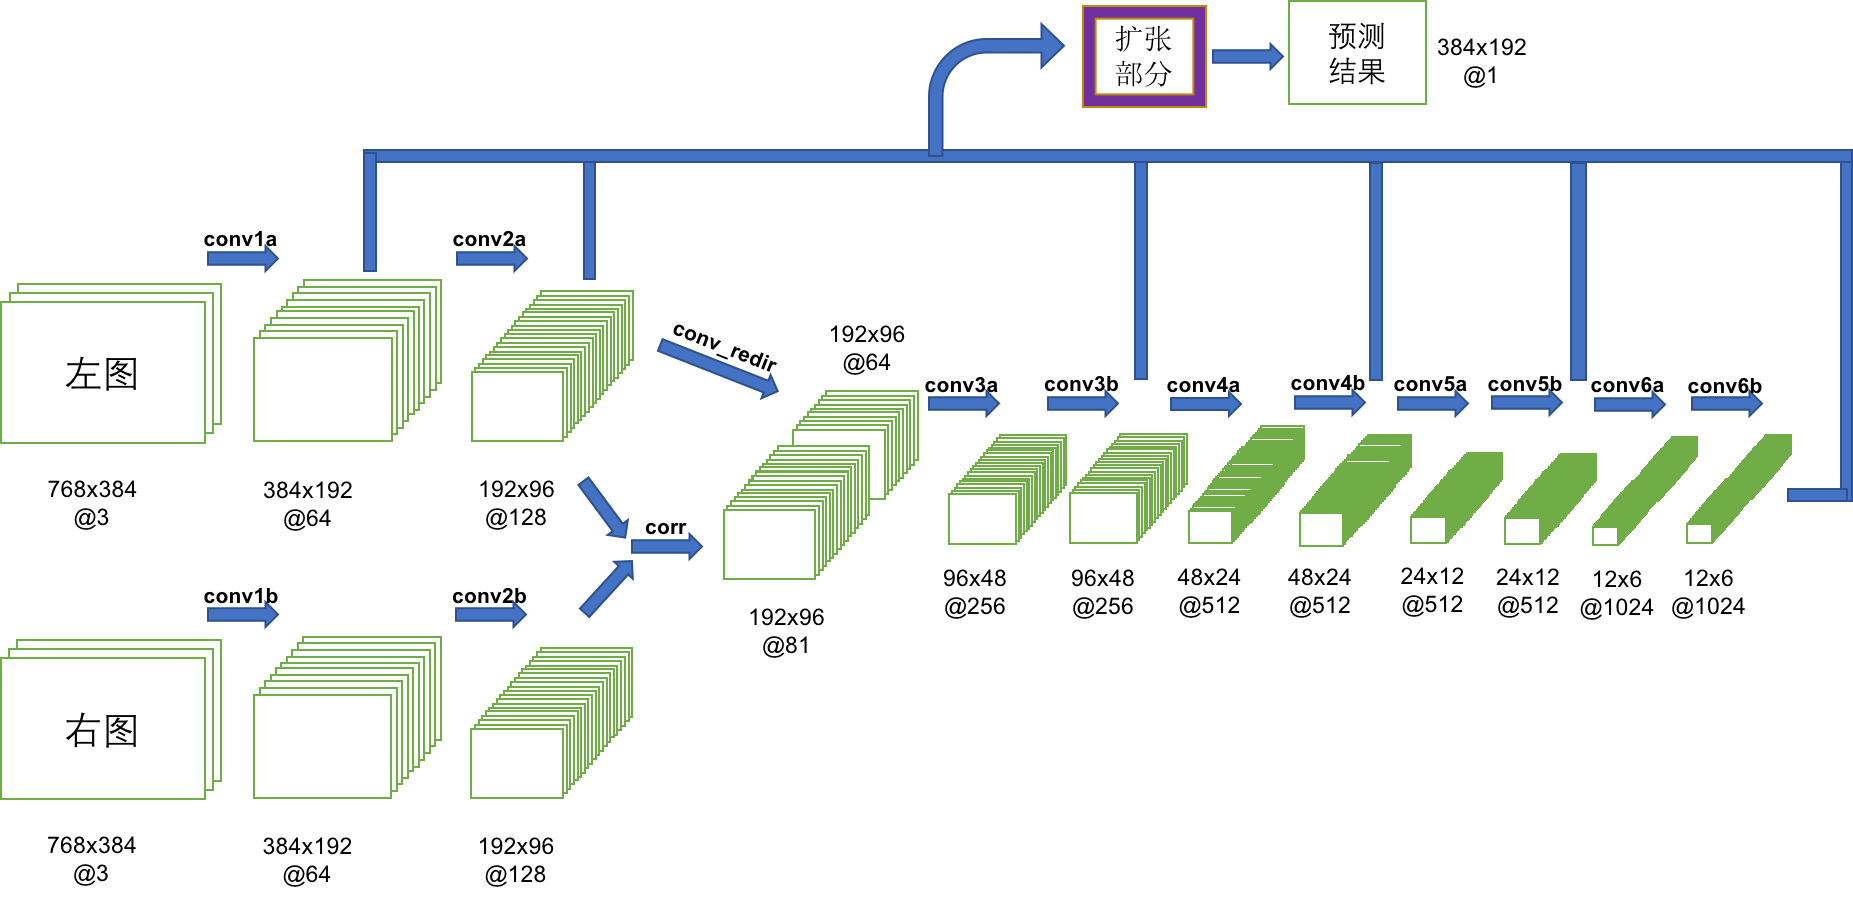
\includegraphics[width=6in]{figures/4_1_dispnetc_architecture}
	\caption{DispNetC网络架构}\label{fig:4_1_DispNetC}
\end{figure}

FlowNet中引入了一个“相关层(correlation layer)”来进行两个特征图之间的比较。假设有两个多通道的特征图
$f_1, f_2: \mathbb{R} \rightarrow \mathbb{R}^c$,$w$,$h$和$c$ 
分别是他们的宽度、高度和通道数。相关层可以让网络比较$f_1$和$f_2$中的每个小块(patch)。为了说明相关层的计算方式,下面只考虑某两个小块之间的比较。取边长为$K=2k+1$的方形小块,第一张特征图中以$x_1$为中心的小块与第二张特征图中以$x_2$为中心的小块的相关量定义为:
\begin{equation}\label{eq:4_1_correlation}  % 前面不要留空行,否则行间距大。
c(\mathbf{x}_1, \mathbf{x}_2) = \sum_{\mathbf{o} \in [-k, k] \times [-k, k]} { \langle \mathbf{f}_1(\mathbf{x}_1 + \mathbf{o}), \mathbf{f}_2(\mathbf{x}_2 + \mathbf{o}) \rangle }
\end{equation}

注意到方程\ref{eq:4_1_correlation}相当于神经网络中步长为1的卷积操作,区别在于这里是用数据与数据进行卷积,而不是使用卷积核,因此并没有可训练的权重参数。

计算$c(\mathbf{x}_1, \mathbf{x}_2)$需要进行$c\cdot K^2$次乘法。而遍历两图中所有的组合方式需要进行$w^2  \cdot h^2$次相关计算,如此大的计算量将无法实现高效的训练和预测。因此出于计算量的考虑,需要限制两图中patch的最大相对位移。设最大位移为$d$,则对于每个$\mathbf{x}_1$,$\mathbf{x}_2$被限制在$\mathbf{x}_1$附近$D=2d+1$的范围内,减小了两图中patch的组合数。另外,FlowNet在相关计算中还加入了步长$s_1, s_2$来进一步减小比较的数量。

由于立体匹配使用的图片是行对齐的,并没有必要进行二维的相关计算,因此简化为水平方向的一维相关计算。取最大相对位移$d$为40个像素,由于在进行相关计算之前图像已经经过了2个步长为2的卷积层,故这里40个像素对应输入图像的160个像素,已经覆盖了足够大的视差范围。相比FlowNet中的二维相关计算,采用一维相关计算大大减小了计算量,而且较FlowNet覆盖了更大的相对位移范围,同时因为不需使用步长,获得了更精细的采样。实际操作中,每个patch取为1个像素。因为加入了相关层,我们称这种网络结构为DispNetC。

%------------------------------------------------------------------------------------
\subsubsection{扩张部分}
扩张部分的主要结构是上卷积层(upconvolutional layer),由去池化(unpooling,与池化相对)和卷积组成。这种网络层已被多次使用过\cite{zeiler2011adaptive, zeiler2014visualizing, goodfellow2014generative}。为了获得精细的预测结果,我们对特征图应用上卷积,并将其和收缩部分中对应的特征图、以及上一层的较粗糙的预测结果拼接起来。这样既保留了从更粗糙的特征图传递过来的高级信息,也保留了更低网络层的特征图提供的精细局部信息。每一次上卷积使预测结果的分辨率增加一倍,一共重复4次上卷积,最终得到的预测结果的分辨率是输入图像的四分之一,宽度和高度都是原图的一半。对网络输出的结果使用插值方法即可获得与输入图像相同的分辨率。根据\cite{dosovitskiy2015flownet}的实验,继续增加上卷积层来细化预测结果相比使用双线性插值方法并不能显著提高预测精度,但由于视差必须取整数,我们使用最近邻插值来得到输入分辨率的结果。扩张部分的结构如图\ref{fig:4_1_DispNet_expanding_part}所示。

\begin{figure}[!htb]
	\centering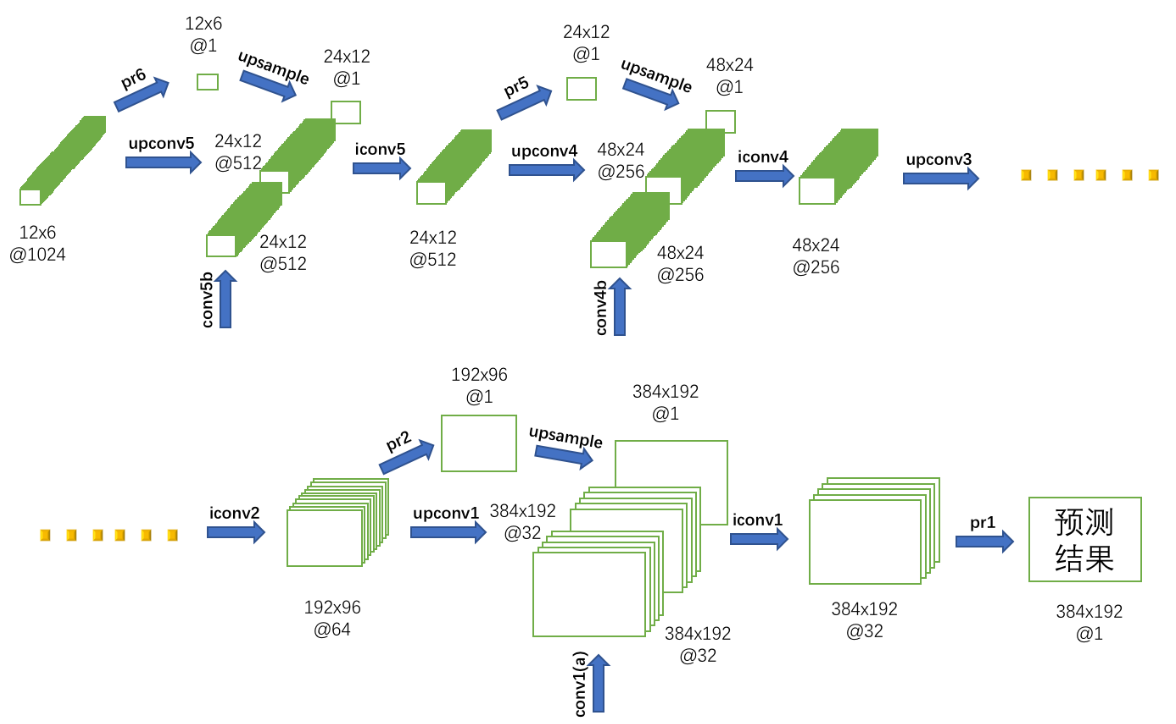
\includegraphics[width=6in]{figures/4_1_dispnet_expanding_part.png}
	\caption{DispNetC扩张部分结构}\label{fig:4_1_DispNet_expanding_part}
\end{figure}

DispNet网络结构的详细参数见表\ref{tab:4_1_DispNet_architecture}。收缩部分包括conv1到conv6b。扩张部分中,上卷积层(upconvN)、卷积层(iconvN,  prN)和代价层(loss)交替出现。最终模型预测的视差图为pr1层的输出。
DispNetC与基础架构的区别存在于前三层。只需要将基础架构的前两层(conv1, conv2)平均拆分为权值共享的两部分,conv1a/b层的输入通道数减小为3。conv2a/b层经过相关层(corr)后的输出通道数为$2d+1=81$,和con2a通过卷积重定向层(conv\_redir)后的结果拼接在一起,再通过conv3a将输出通道数与基础架构中conv3a的输出进行统一,其余部分与基础架构完全一致。
% leaky relu要不要介绍???
网络收缩部分每个卷积层使用的激活函数为Leaky ReLU,扩张部分不使用激活函数。

\begin{table}[htbp] % 这两个表格是不是应该放到附录里去。算了。
	\centering
	\caption{DispNet网络结构详细参数}
	\label{tab:4_1_DispNet_architecture}
	\begin{scriptsize}   % tiny, scriptsize, footnotesize, small.
		\begin{tabular}{|l|c c c|c c|c|}\hline
			网络层 & 卷积核 & 步长 & 输入/输出通道数 & 输入分辨率 & 输出分辨率 & 该层输入 \\\hline
			%---------------------------------------------------------
			conv1    & 7x7 & 2 & 6/64                & 768x384 & 384x192 & 左右图像 \\
			conv2    & 5x5 & 2 & 64/128           & 384x192  & 192x96    & conv1 \\
			conv3a & 5x5 & 2 & 128/256         & 192x96     & 96x48      & conv2 \\
			conv3b & 3x3 & 1 & 256/256        & 96x48       & 96x48      & conv3a\\
			conv4a & 3x3 & 2 & 256/512        & 96x48        & 48x24      & conv3b \\
			conv4b & 3x3 & 1 & 512/512         & 48x24        & 48x24       & conv4a \\
			conv5a & 3x3 & 2 & 512/512         & 48x24        & 24x12        & conv4b \\
			conv5b & 3x3 & 1 & 512/512         & 24x12          & 24x12       & conv5a \\
			conv6a & 3x3 & 2 & 512/1024     & 24x12          & 12x6          & conv5b \\
			conv6b & 3x3 & 1 & 1024/1024  & 12x6             & 12x6          & conv6a \\\hline
			%---------------------------------------------------------
			pr6+loss6 & 3x3 & 1 & 1024/1 & 12x6 & 12x6 & conv6b \\\hline
			%---------------------------------------------------------
			upconv5    & 4x4 & 2 & 1024/512  & 12x6        & 24x12    & conv6b \\
			iconv5        & 3x3 & 1 & 1025/512  & 24x12      & 24x12    & upconv5+pr6+conv5b \\
			pr5+loss5  & 3x3 & 1 & 512/1         & 24x12      & 24x12    & iconv5 \\
			upconv4    & 4x4 & 2 & 512/256   & 24x12      & 48x24    & iconv5 \\
			iconv4        & 3x3 & 1 & 769/256  & 48x24     & 48x24    & upconv4+pr5+conv4b \\
			pr4+loss4 & 3x3 & 1  & 256/1       & 48x24     & 48x24    & iconv4 \\
			upconv3    & 4x4 & 2 & 256/128  & 48x24     & 96x48    & iconv4 \\
			iconv3        & 3x3 & 1 & 385/128  & 96x48    & 96x48    & upconv3+pr4+conv3b \\
			pr3+loss3 & 3x3 & 1 & 128/1        & 96x48    & 96x48    & iconv3 \\
			upconv2    & 4x4 & 2 & 128/64    & 96x48    & 192x96   & iconv3 \\
			iconv2        & 3x3 & 1 & 193/64   & 192x96   & 192x96   & upconv2+pr3+conv2 \\
			pr2+loss2  & 3x3 & 1 & 64/1        & 192x96   & 192x96    & iconv2 \\
			upconv1     & 4x4 & 2 & 64/32    & 192x96    & 384x192 & iconv2 \\
			iconv1        & 3x3 & 1 & 93/32     &384x192  & 384x192 & upconv1+pr2+conv1 \\
			pr1+loss1  & 3x3 & 1 & 32/1         & 384x192 & 384x192 & iconv1 \\\hline
			%---------------------------------------------------------
		\end{tabular}
    \end{scriptsize}
\end{table}

\begin{table}[htbp]
	\centering
	\caption{DispNetC与基础架构差异部分的详细参数}
	\label{tab:4_1_DispNetC_architecture}
	\begin{scriptsize}
		\begin{tabular}{|l|c c c|c c|c|}\hline
			网络层  & 卷积核 & 步长 & 输入/输出通道数 & 输入分辨率 & 输出分辨率 & 该层输入 \\\hline
			%---------------------------------------------------------
			conv1a             & 7x7 & 2 & 3/64                & 768x384 & 384x192 & 左图 \\
			conv1b             & 7x7 & 2 & 3/64                & 768x384 & 384x192 & 右图 \\
			conv2a             & 5x5 & 2 & 64/128           & 384x192  & 192x96    & conv1a \\
			conv2b             & 5x5 & 2 & 64/128           & 384x192  & 192x96    & conv1b \\
			conv\_redir      & 1x1 & 1 & 128/64            & 192x96    & 192x96    & conv2a \\
			corr                   & --   &  - & 128/81            & 192x96    & 192x96    & conv2a+conv2b \\
			conv3a            & 5x5 & 2 & 64+81/256    & 192x96    & 96x48      & corr+conv\_redir \\\hline
		\end{tabular}
	\end{scriptsize}
\end{table}

根据论文\cite{mayer2016large}给出的结果,DispNetC的效果优于DispNet,而运行时间上两者并没有明显差异,因此本文采用DispNetC网络结构。

%------------------------------------------------------------------------------------
\section{网络训练}
网络的训练是通过端到端的方式进行的,以成对的图像作为网络输入,使用真实视差图(ground truth)对网络预测输出的视差图进行监督。监督学习需要大量的样本数据,然而实际生活中很难获得大量场景的真实视差,这给网络模型的训练带来了很大的困难。为了解决这个矛盾,本文使用FlyingThings3D和KITTI 2个数据集进行训练。

\subsection{FlyingThings3D和KITTI数据集}
FlyingThings3D\cite{mayer2016large}是使用开源的三维动画制作软件Blender生成的场景流(scene flow)数据集,其中也包含立体RBG图像及其视差的真实值。对于每个生成的场景,直接提取每个像素的三维坐标,根据虚拟双目相机的配置参数计算出视差真值。因为渲染引擎掌握生成场景中所有点的信息,故即使对于遮挡区域也能获得其视差真值,即视差的ground truth是100\%稠密的。图像中的场景是生活中常见的各种物品在空中沿随机三维轨迹飞行。FlyingThings3D数据集是专门用来训练大型卷积神经网络的,共包含32872组训练数据和3055组测试数据。

KITTI数据集有两部分,一部分是2012年制作的\cite{Geiger2012},另一部分公布于2015年\cite{Menze_2015_CVPR}。KITTI数据集包含道路场景的双目立体视频,视频是通过在一辆汽车上安装一对标定好的相机获取的,而视差真值是利用一个三维激光扫描仪得到的。KITTI包含了真实世界中的数据,但只有场景中静止部分的数据是有效的,另外由于激光扫描仪具有一定的距离和高度的工作范围限制,数据集只能提供稀疏的视差真值。KITTI2015包含200组训练数据和200组测试数据,只有训练集提供了ground truth;本文中的实验未使用KITTI2012,因为其只提供了灰度图像。


\subsection{网络训练过程}
KITTI数据集包含真实场景的数据,但其数据量较小,且ground truth是稀疏的;而Flyingthings3D中的场景是人工合成的,但其数据量巨大且包含100\%稠密的视差真值。因此,我们首先使用FlyingThings3D来训练网络,在网络学习到从图像中预测视差的模式后,再在KITTI2015数据集上进行微调(finetune),从而获得对真实立体图像的匹配效果。

训练和测试使用的数据均来自两个数据集中提供了ground truth的部分。
在Flyingthings3D上训练时,训练集包含22890组数据,测试集包含4370组数据;在KITTI2015上训练时,分别使用前160组和后40组数据作为训练集和测试集。图像输入网络前需进行预处理:使用最近邻插值调整分辨率与网络输入一致(768x384);左右图的RGB像素值范围从$[0, 255]$映射到$[-1, 1]$;视差图像素值保持为$[0, 255]$,但需要除以图像尺寸缩放的系数,因为图像尺寸改变会导致视差值的改变。

本文使用TensorFlow\cite{abadi2016tensorflow}作为搭建、训练网络模型的软件平台。
% TODO: TensorFlow只介绍一次,如果第三章写目标检测,就不用放在这里了!
% TODO: Adam有必要介绍一下公式吗?
% https://zhuanlan.zhihu.com/p/22252270
% http://ruder.io/optimizing-gradient-descent/index.html#adam
梯度下降使用Adam(Adaptive moment estimation,自适应矩估计)优化器\cite{kingma2014adam},参数设置:$\beta_1=0.9, \beta_2=0.999$。
% 实际上程序里beta_2是0.99。。。
Adam算法根据损失函数对每个参数的梯度的一阶矩估计和二阶矩估计动态调整每个参数的学习率,其优点在于经过偏置校正后,学习率在每次迭代中都有个确定的范围,使得参数变化比较平稳。更新规则为:
\begin{equation}\label{eq_4_2_Adam}
\begin{cases}
m_t = \beta_1 m_{t-1} + (1 - \beta_1)g_t \\
v_t = \beta_2 v_{t-1} + (1 - \beta_2) g_t^2 \\
\hat{m}_t = \frac{m_t}{1 - \beta_1^t} \\
\hat{v}_t = \frac{v_t}{1 - \beta_2^{t}} \\
\theta_{t+1} = \theta_t - \frac{\hat{m}_t}{\sqrt{\hat{v_t} + \epsilon}} \eta
\end{cases}
\end{equation}
其中,$g_t$为t时刻的梯度,$m_t$、$v_t$分别是梯度的一阶和二阶矩估计,$\hat{m_t}$、$\hat{n_t}$是偏置校正后的矩估计,$\eta$为学习率,$\theta$为更新的参数。可见$\frac{\hat{m_t}}{\sqrt{\hat{v_t}}+\epsilon}$对学习率形成了一个动态的约束。

学习率初始化为$\eta=0.0001$,在训练迭代400k次后每200k减半。
损失函数定义为6个尺度下的损失的加权和。每个尺度下的损失定义为该尺度下的预测结果$P_n$和视差真值$G_n$的绝对误差和。各尺度下的视差真值是由网络输入的视差图通过最近邻插值得到的。
另外加入L2正则化项,权重取为$\alpha=0.0004$,用于防止模型过拟合,提高泛化能力。
\begin{equation}\label{eq:4_2_loss_all}
loss = \sum_{n=1}^{6}{w_n * loss_n} + \alpha ||\theta||_2^2
\end{equation}
\begin{equation}\label{eq:4_2_loss_single}
loss_n = \sum_{i=1}^{H_n}\sum_{j=1}^{W_n}{|P_n(i, j) - G_n(i, j)|}
\end{equation}
公式中$w_n$表示尺度$n$下的损失权重,$\alpha||\theta||_2^2$为正则化项,$W_n$和$H_n$分别为尺度$n$下图像的宽和高。

由于网络比较深,且收缩部分和扩张部分之间存在直接的连接,如果同时计入6个尺度的损失,网络中低层的梯度方向受到多个损失的影响,损失函数可能无法高效地下降。为损失权重设计一个进度表(表\ref{tab:4_2_loss_weight_schedule})可以改善这种情况:开始训练时,设置最小尺度的loss6的权重为1,其余尺度的loss权重为0;随着训练的进行,逐渐增大高分辨率尺度损失的权重,降低低分辨率尺度损失的权重。这样使得网络先学习到粗糙的表示,然后向更精细的方向发展,同时损失函数不再对中低层特征进行限制。

\begin{table}[htb]
	\centering
	\caption{损失函数权重进度表}
	\label{tab:4_2_loss_weight_schedule}
	\begin{small} %{scriptsize}
		\begin{tabular}{|l|cccccc|}\hline
			迭代次数  & $w_1$ & $w_2$ & $w_3$ & $w_4$ & $w_5$ & $w_6$ \\\hline
			%---------------------------------------------------------
			(0, 50k]           & 0 & 0 & 0 & 0 & 0.2 & 1 \\
			(50k, 100k]     & 0 & 0 & 0 & 0.2 & 1 & 0.5 \\
			(100k, 150k]    & 0 & 0 & 0.2 & 1 & 0.5 & 0 \\
			(150k, 200k]    & 0 & 0.2 & 1 & 0.5 & 0 & 0 \\
			(200k, 250k]    & 0.2 & 1 & 0.5 & 0 & 0 & 0  \\
			(250k, 300k]    & 1 & 0.5 & 0 & 0 & 0 & 0  \\
			(300k, --)          & 1 & 0 & 0 & 0 & 0 & 0 \\\hline
		\end{tabular}
	\end{small} %{scriptsize}
\end{table}

%------------------------------------------------------------------------------------
\section{实验结果}
本实验的运行环境与目标检测实验相同。

\subsection{评价指标}
目前立体匹配领域使用最多的评价指标是平均视差误差(Endpoint error),其定义为预测结果中各点的视差值与视差真值的绝对误差均值:
\begin{equation}\label{eq:4_3_endpoint_error}
e = \frac{1}{M} \left( \sum_{\mathbf{p} \in \mathbf{A}} | d(\mathbf{p}) - d_{gt}(\mathbf{p}) | \right)
\end{equation}
其中,$\mathbf{A}$表示真实视差图中有效视差点的集合(即具有非零像素值的点),M为有效视差点的数量,$d(\mathbf{p})$和$d_{gt}(\mathbf{p})$分别表示计算所得的视差图和真实视差图中点$\mathbf{p}$的视差值。

KITTI2015中使用了另一种评价指标:平均错误率(D),或称为误匹配像素百分比(PBM, Percentage of Bad Matching)。其定义为匹配结果中视差值误差同时大于3像素和视差真值的5\%的像素点所占比例:
\begin{equation}\label{eq:4_3_D1_error}
D = \frac{1}{M}\left( \sum_{\mathbf{p} \in \mathbf{A}} \Big[ \big| d(\mathbf{p}) - d_{gt}(\mathbf{p})) \big| > max(3\mathtt{px}, d_{gt}(\mathbf{p}) \times 5\%) \Big] \right)
\end{equation}

下文中提到“误差”时默认指第一种指标,使用第二种指标时会明确指明"D1",1表示误差的计算是在左图上进行的。

\subsection{FlyingThings3D上的实验结果}
使用FlyingThings3D数据集训练1.4e5个迭代,网络的损失函数和训练/测试误差的变化趋势分别如图\ref{fig:4_3_ft3d_loss}和\ref{fig:4_3_ft3d_error}所示(数据已做平滑处理)。训练误差是每轮迭代中batch(4组图片)的平均误差,测试误差是每5000次迭代在整个测试集(4370组图片)上测试得到的平均误差。由图可见,损失函数在1000k次迭代后基本已经收敛,不再有明显的下降;训练误差仍在非常缓慢地下降,但测试误差已经收敛,继续训练只会造成过拟合。
%解释一下为什么200k误差突变。
% TODO:这个脑残的loss weight schedule怎么洗白啊。。。
训练/测试误差在200k次迭代时的突变是由于损失函数权重的调整造成的。对照表\ref{tab:4_2_loss_weight_schedule},200k之前loss1未计入loss,而误差是在loss1对应尺度(384x192)下定义的,故误差并没有明显的下降。但前200k的训练并不是无效的,因为损失函数获得了有效的下降。

%--------------------- 每张图一行
%\begin{figure}[!htbp]
%	\centering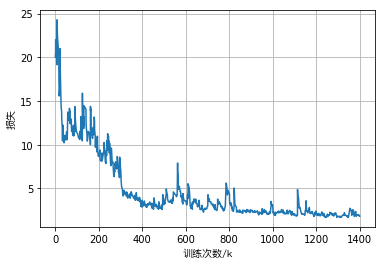
\includegraphics[width=4in]{figures/4_3_ft3d_loss}
%	\caption{损失函数变化趋势}\label{fig:4_3_ft3d_loss}
%\end{figure}
%\begin{figure}[!htbp]
%	\centering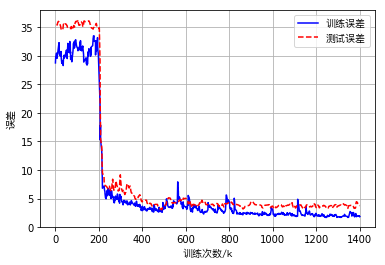
\includegraphics[width=4in]{figures/4_3_ft3d_error}
%	\caption{训练/测试误差变化趋势}\label{fig:4_3_ft3d_error}
%\end{figure}

%--------------------- 2张图同一行
\begin{figure}[htbp]
	\centering
	\begin{minipage}[c]{0.48\textwidth}
		\centering
		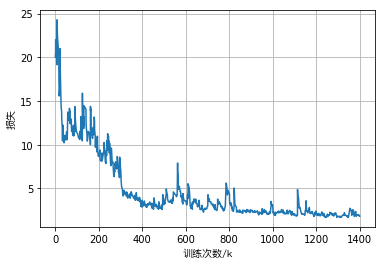
\includegraphics[width=3in]{figures/4_3_ft3d_loss}
		\caption{损失函数变化趋势}\label{fig:4_3_ft3d_loss}
	\end{minipage}
	\hfill
	\begin{minipage}[c]{0.48\textwidth}
		\centering
		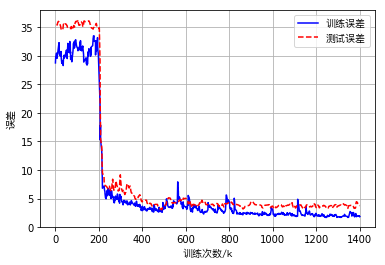
\includegraphics[width=3in]{figures/4_3_ft3d_error}
		\caption{训练/测试误差变化趋势}\label{fig:4_3_ft3d_error}
	\end{minipage}
\end{figure}

训练1400k后,最终的测试误差为: $e = 3.78$px, $D1 = 14.94\%$。
需要说明的是,FlyingThings3D数据集本身存在一些缺陷,其中有些失效的图片,还有无法单纯依靠匹配算法进行匹配的图片(如图\ref{fig:4_3_abnormal}),这些数据难以从数据集中剔除,因此测试结果的误差会比应用在现实场景中时偏大。

% abnormal image pairs
\begin{figure}[!htbp]
	\centering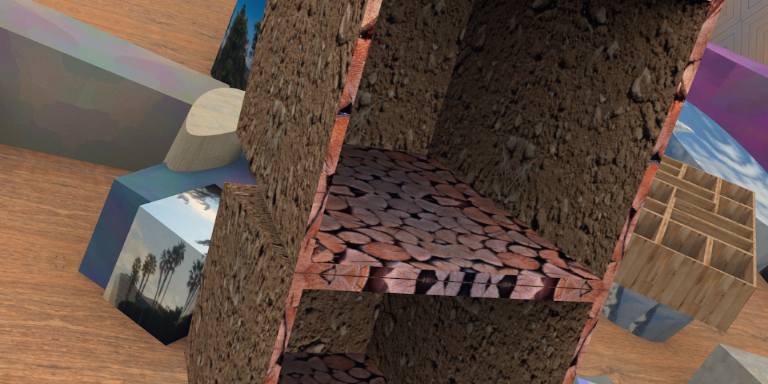
\includegraphics[width=2.5in]{figures/4_3_abnormal_imgs/l_003}
	\hspace{20pt}
	\centering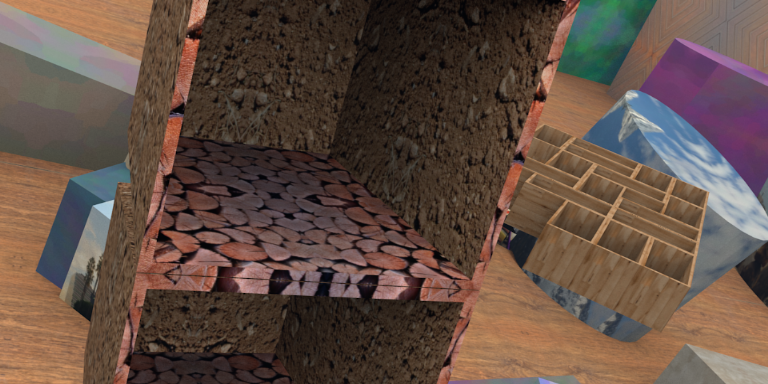
\includegraphics[width=2.5in]{figures/4_3_abnormal_imgs/r_003}
	\caption{FlyingThings3D中难以匹配的图片}\label{fig:4_3_abnormal}
\end{figure}

为了体现算法的效果,我们与两种优秀的传统立体匹配算法SGM\cite{Hirschmuller08}、SPS-St\cite{yamaguchi2014}进行比较。图\ref{fig:4_3_ft3d_cmp_result}给出了应用三种算法在FlyingThings3D部分测试图片上的匹配结果。


% 三种算法在ft3d上的匹配结果对比图. 
\begin{figure}[!htb]
	% 3组占不满一页,4组放不开,蛋疼。‘!’忽略美学标准,强制和文字凑一页。
	%>>>>>>>>>>>>>>>>>>>>第1组>>>>>>>>>>>>>>>>>>>>
	%----------------------第1行-----------------------
	\begin{minipage}{0.3\linewidth}
		\centerline{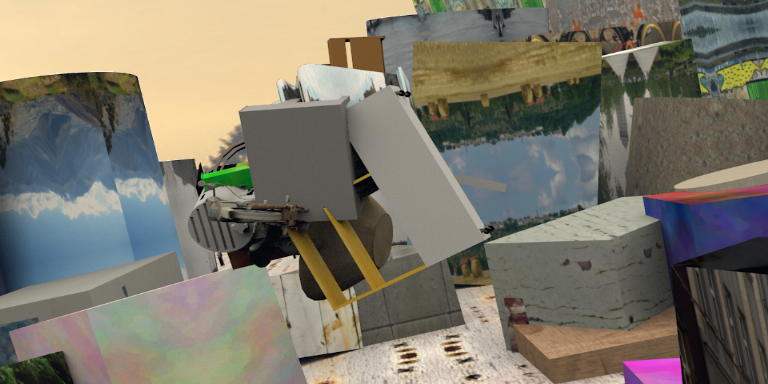
\includegraphics[width=2in]{figures/cmp_ft3d/l_000}}
		\vspace{-10pt}
		\centerline{左图}
	\end{minipage}
	\hfill
	\begin{minipage}{.3\linewidth}
		\centerline{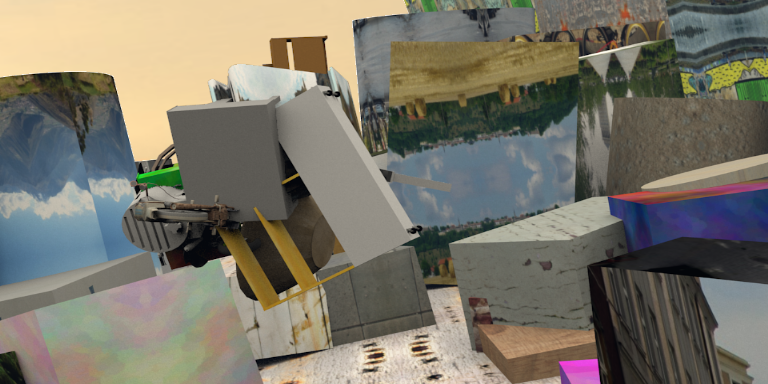
\includegraphics[width=2in]{figures/cmp_ft3d/r_000}}
		\vspace{-10pt}
		\centerline{右图}
	\end{minipage}
	\hfill
	\begin{minipage}{0.3\linewidth}
		\centerline{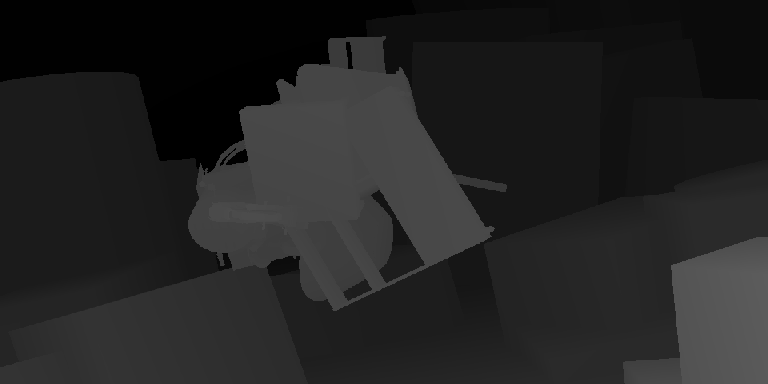
\includegraphics[width=2in]{figures/cmp_ft3d/gt_000}}
		\vspace{-10pt}
		\centerline{ground truth}
	\end{minipage}
	\vfill
	%----------------------第2行----------------------
	\begin{minipage}{0.3\linewidth}
		\centerline{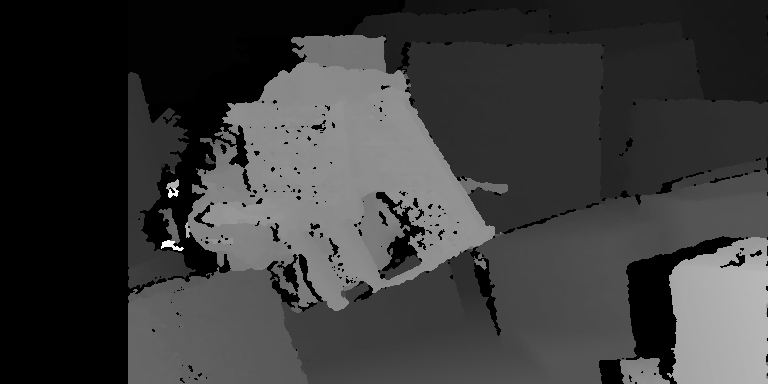
\includegraphics[width=2in]{figures/cmp_ft3d/sgm_000}}
		\vspace{-10pt}
		\centerline{SGM}
	\end{minipage}
	\hfill
	\begin{minipage}{0.3\linewidth}
		\centerline{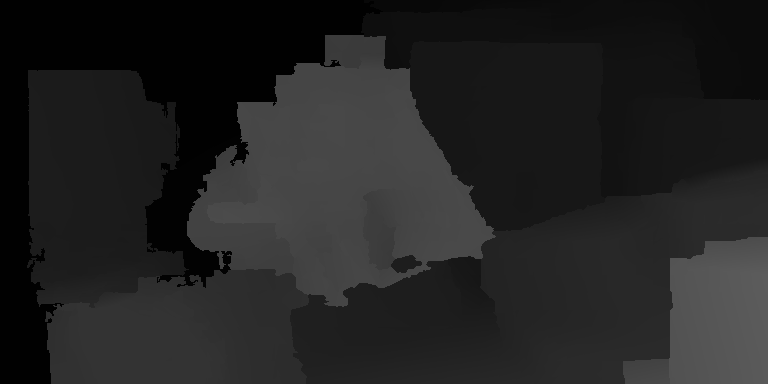
\includegraphics[width=2in]{figures/cmp_ft3d/sps_000}}
		\vspace{-10pt}
		\centerline{SPS-St}
	\end{minipage}
	\hfill
	\begin{minipage}{0.3\linewidth}
		\centerline{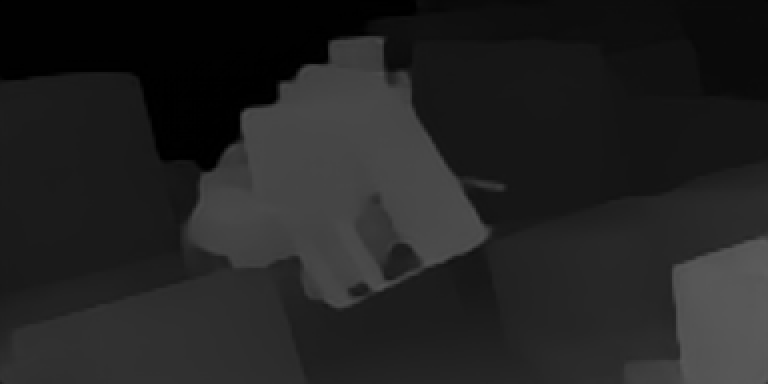
\includegraphics[width=2in]{figures/cmp_ft3d/pred_000}}
		\vspace{-10pt}
		\centerline{DispNetC}
	\end{minipage}
	%<<<<<<<<<<<<<<<<<<<<第1组<<<<<<<<<<<<<<<<<<<<
	%>>>>>>>>>>>>>>>>>>>>第2组>>>>>>>>>>>>>>>>>>>>
	%----------------------第1行-----------------------
		\begin{minipage}{0.3\linewidth}
		\centerline{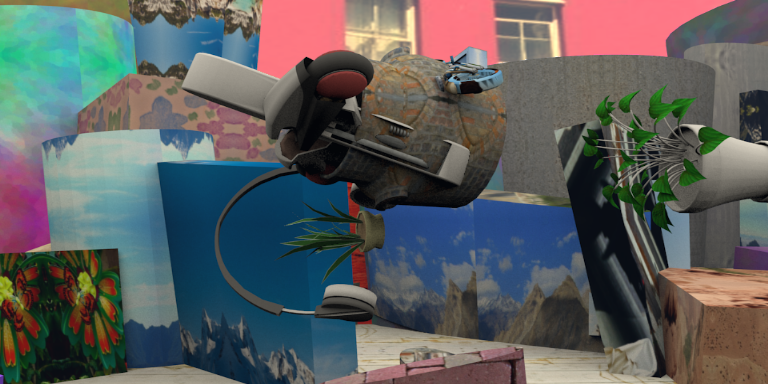
\includegraphics[width=2in]{figures/cmp_ft3d/l_005}}
		\vspace{-10pt}
		\centerline{左图}
	\end{minipage}
	\hfill
	\begin{minipage}{.3\linewidth}
		\centerline{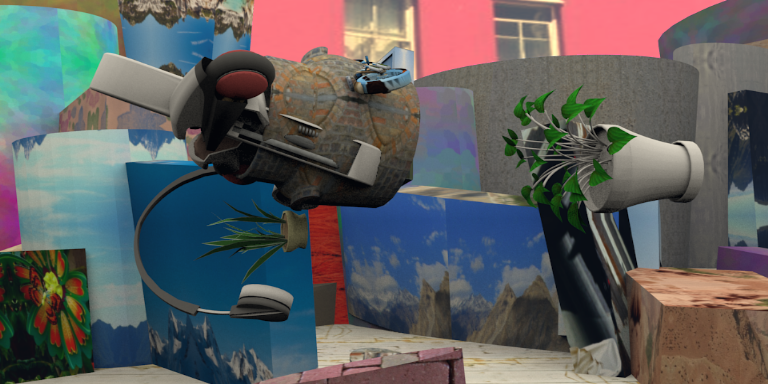
\includegraphics[width=2in]{figures/cmp_ft3d/r_005}}
		\vspace{-10pt}
		\centerline{右图}
	\end{minipage}
	\hfill
	\begin{minipage}{0.3\linewidth}
		\centerline{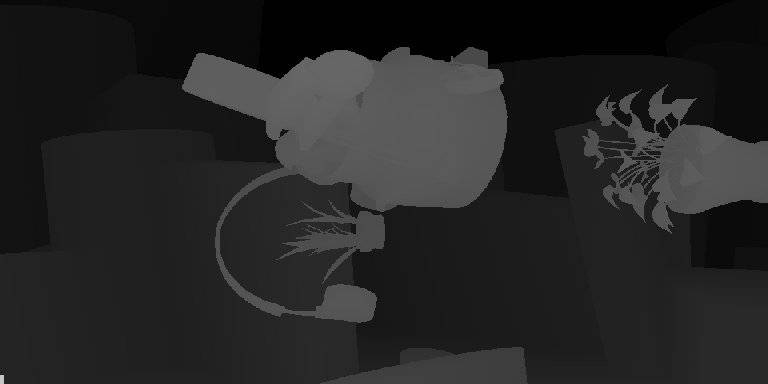
\includegraphics[width=2in]{figures/cmp_ft3d/gt_005}}
		\vspace{-10pt}
		\centerline{ground truth}
	\end{minipage}
	\vfill
	%----------------------第2行-----------------------
	\begin{minipage}{0.3\linewidth}
		\centerline{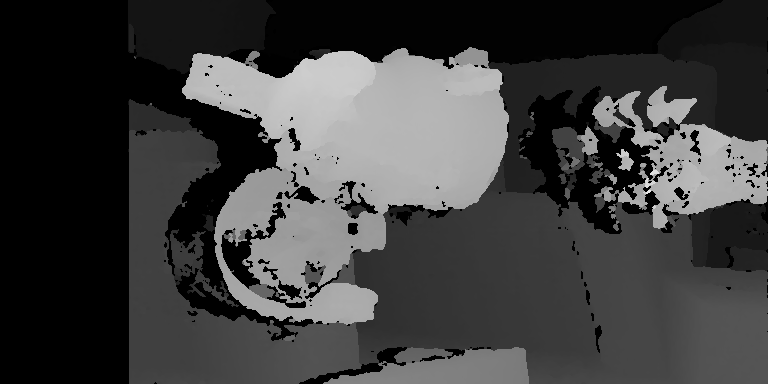
\includegraphics[width=2in]{figures/cmp_ft3d/sgm_005}}
		\vspace{-10pt}
		\centerline{SGM}
	\end{minipage}
	\hfill
	\begin{minipage}{0.3\linewidth}
		\centerline{
\includegraphics[width=2in]{figures/cmp_ft3d/sps_005}}
		\vspace{-10pt}
		\centerline{SPS-St}
	\end{minipage}
	\hfill
	\begin{minipage}{0.3\linewidth}
	\centerline{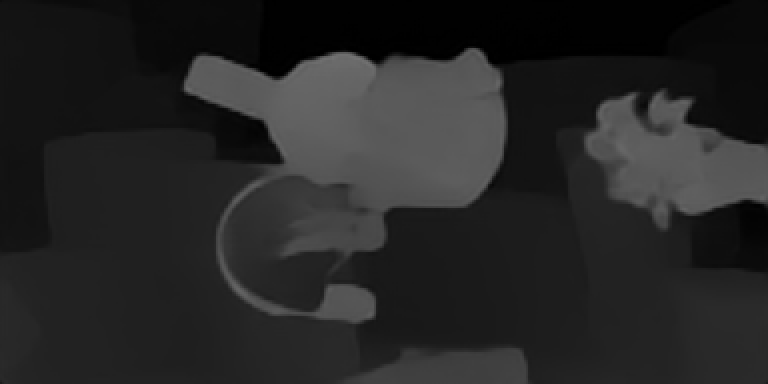
\includegraphics[width=2in]{figures/cmp_ft3d/pred_005}}
	\vspace{-10pt}
	\centerline{DispNetC}
\end{minipage}
	%<<<<<<<<<<<<<<<<<<<<第2组<<<<<<<<<<<<<<<<<<<<
	%>>>>>>>>>>>>>>>>>>>>第3组>>>>>>>>>>>>>>>>>>>>
	%----------------------第1行-----------------------
	\begin{minipage}{0.3\linewidth}
		\centerline{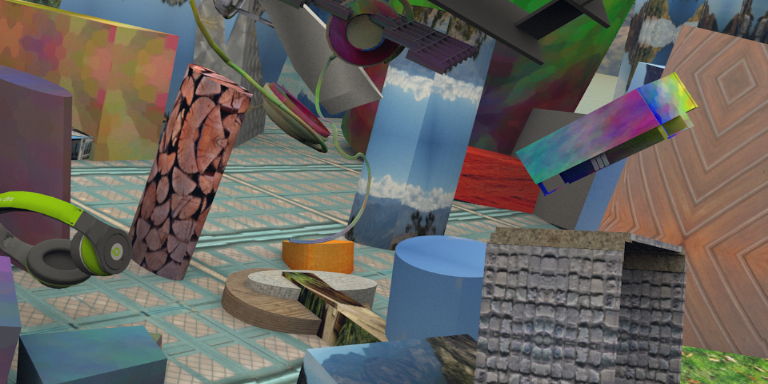
\includegraphics[width=2in]{figures/cmp_ft3d/l_039}}
		\vspace{-10pt}
		\centerline{左图}
	\end{minipage}
	\hfill
	\begin{minipage}{.3\linewidth}
		\centerline{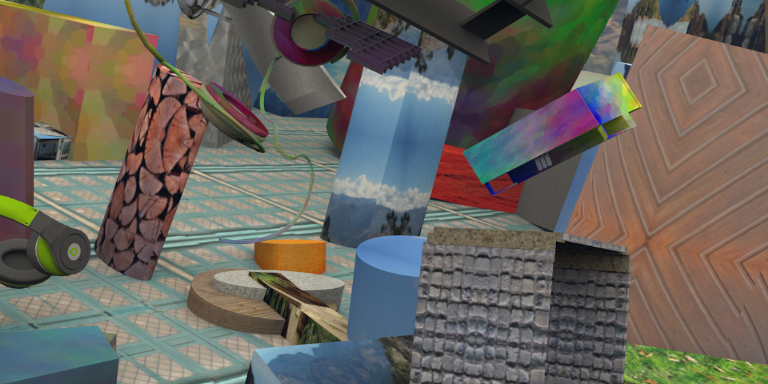
\includegraphics[width=2in]{figures/cmp_ft3d/r_039}}
		\vspace{-10pt}
		\centerline{右图}
	\end{minipage}
	\hfill
	\begin{minipage}{0.3\linewidth}
		\centerline{
\includegraphics[width=2in]{figures/cmp_ft3d/gt_039}}
		\vspace{-10pt}
		\centerline{ground truth}
	\end{minipage}
	\vfill
	%----------------------第2行-----------------------
	\begin{minipage}{0.3\linewidth}
		\centerline{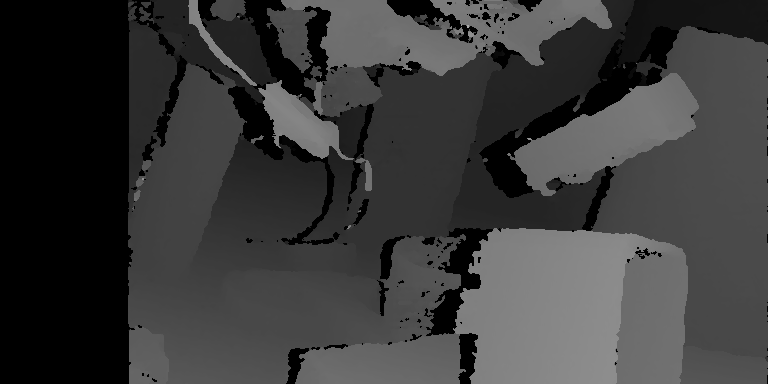
\includegraphics[width=2in]{figures/cmp_ft3d/sgm_039}}
		\vspace{-10pt}
		\centerline{SGM}
	\end{minipage}
	\hfill
	\begin{minipage}{0.3\linewidth}
		\centerline{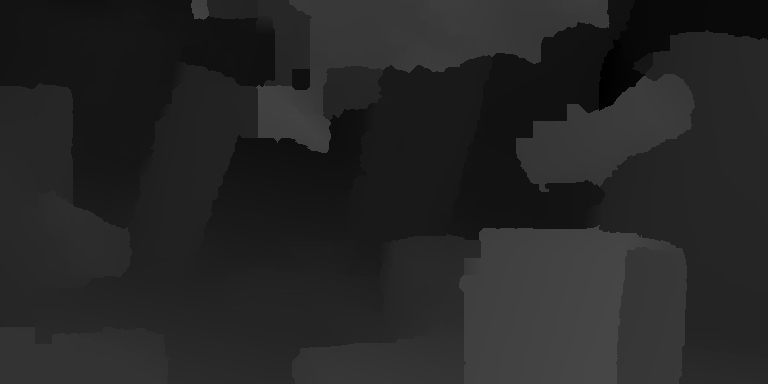
\includegraphics[width=2in]{figures/cmp_ft3d/sps_039}}
		\vspace{-10pt}
		\centerline{SPS-St}
	\end{minipage}
	\hfill
	\begin{minipage}{0.3\linewidth}
		\centerline{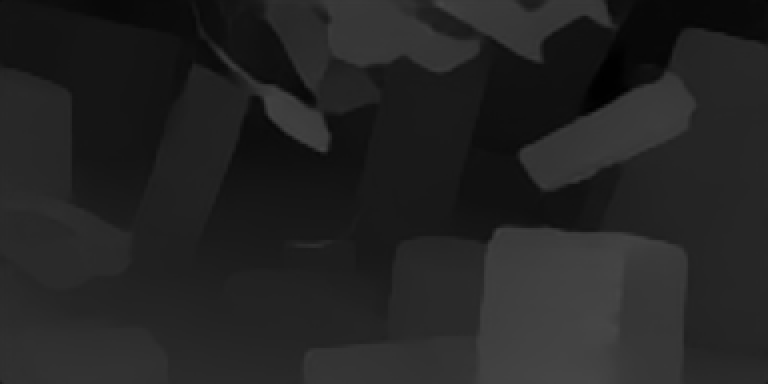
\includegraphics[width=2in]{figures/cmp_ft3d/pred_039}}
		\vspace{-10pt}
		\centerline{DispNetC}
	\end{minipage}
	%<<<<<<<<<<<<<<<<<<<<第3组<<<<<<<<<<<<<<<<<<<<
	\caption{DispNetC, SGM和SPS-St在FlyingThings3D部分测试图片上的匹配结果}
	\label{fig:4_3_ft3d_cmp_result}
\end{figure}

%--------------------- 优缺点 --------------------- 
对比三种算法的结果,可以看出本文算法具有以下优点:

(1)
%匹配精度高,%这句话说不出来了。。
对全局信息的利用较好,可以较准确地推理出缺少纹理区域和遮挡区域的视差,生成100\%稠密的视差图。SGM算法得到的结果中有很多匹配失败的点,无法得到被遮挡区域的视差,而且视差搜索范围越大得到的视差图越小(左侧黑色区域越大)。SPS-St算法由于使用了倾斜平面模型(slanted plane model),能得到一部分遮挡区域的视差,但丢失大量细节,前景膨胀严重,在视差不连续处表现较差。

(2)
运行速度快。由于大部分计算在GPU上进行,DispNetC网络在每次输入一组图片时前向传播速度约为0.05s,具有较好的实时性;而SGM的运行时间与最大视差范围、窗口尺寸等参数有关,视差搜索范围和匹配窗口越大,运行时间越长,一般在0.2s以上;SPS-St采用SGM作为初始步骤,计算量更大,运行时间约为2s,完全无法应用于有实时性要求的场景。

(3)
应用简便,通用性好,鲁棒性强。SGM等算法需要人工设置搜索范围、匹配窗口尺寸等参数以适应不同的应用场景,而DispNetC完全从图像数据中学习匹配规律,网络训练完成后可直接应用,不需调参。通过在训练时对训练数据进行数据增强,可以使网络在光照变化等方面具备较好的鲁棒性。
% 鲁棒性?

当然,DispNetC算法也存在缺点,其对于细节的预测不够准确,视差不连续处比较模糊。另外作为深度学习算法,其训练时间长,网络模型较大,对计算和存储设备提出了较高的要求,一定程度上限制了其应用场景。

\subsection{KITTI2015上的实验结果}
Flyingthings3D是人工合成的数据集,与真实场景具有一定的差异,因此我们在训练完成后使用KITTI2015训练集进行网络参数的微调(finetune),以更好地应用于现实中。微调训练使用前160组图片,共进行200k次迭代;测试使用后40组图片。微调过程中损失函数和误差的变化趋势如图\ref{fig:4_3_kitti_loss}和\ref{fig:4_3_test_error}所示。由于训练集数据量很小,网络在20k次迭代后测试误差已经基本不再下降。

%--------------------- 2张图同一行
\begin{figure}[htbp]
	\centering
	\begin{minipage}[c]{0.48\textwidth}
		\centering
		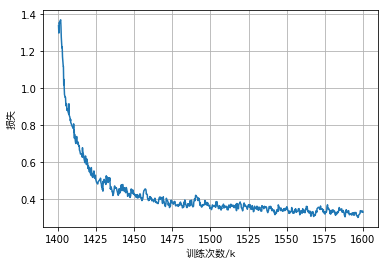
\includegraphics[width=3in]{figures/4_3_kitti_loss}
		\caption{KITTI2015上的损失函数变化趋势}\label{fig:4_3_kitti_loss}
	\end{minipage}
	\hfill
	\begin{minipage}[c]{0.48\textwidth}
		\centering
		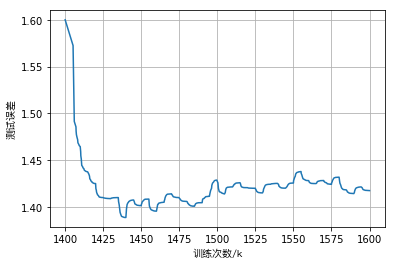
\includegraphics[width=3in]{figures/4_3_kitti_test_error}
		\caption{KITTI2015上的测试误差变化趋势}\label{fig:4_3_test_error}
	\end{minipage}
\end{figure}

类似上一小节,我们同时给出DispNetC、SGM和SPS-St在KITTI数据集上的匹配效果,如图\ref{fig:4_3_kitti_cmp_result}。另外,表\ref{tab:4_3_cmp_kitti}给出了多种匹配算法的误差比较\cite{Menze_2015_CVPR}\cite{陈拓2017CCNN}。本实验训练的DispNetC网络模型的匹配准确度明显优于SGM、AD、BM等算法;而且在运行时间方面,DispNetC远快于其他方法。
% TODO: 补上数据。% 略差于(还是好于?)SPS-St.  先不跟你比了。。

% 三种算法在kitti上的匹配结果对比图.
\begin{figure}[!htb]
	% 一页只能放4组。备选5组:11, 29,31, 32, 97。11和29场景相似,选一个。
	%>>>>>>>>>>>>>>>>>>>>第1组>>>>>>>>>>>>>>>>>>>>
	%----------------------第1行-----------------------
	\begin{minipage}{0.48\linewidth}
		\centerline{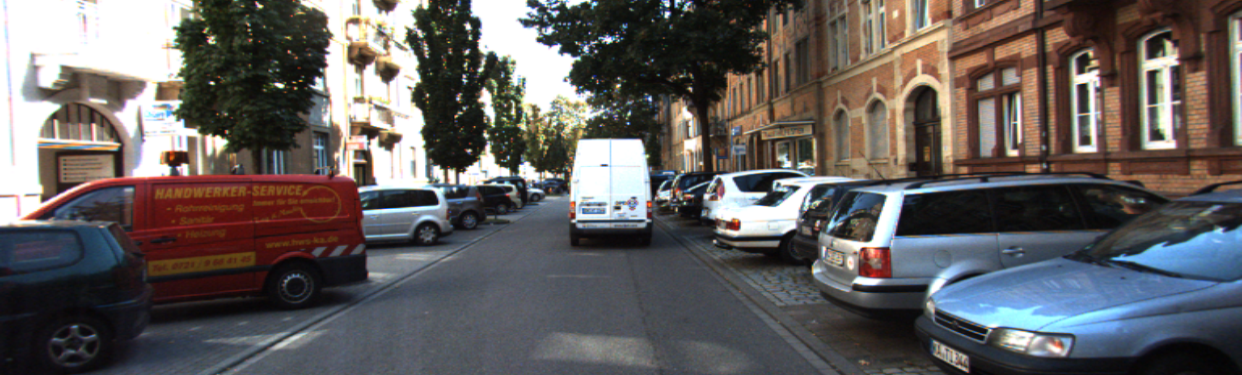
\includegraphics[width=3in]{figures/cmp_kitti/l_029}}
		\vspace{-10pt}
		\centerline{左图}
	\end{minipage}
	\hfill
	\begin{minipage}{0.48\linewidth}
		\centerline{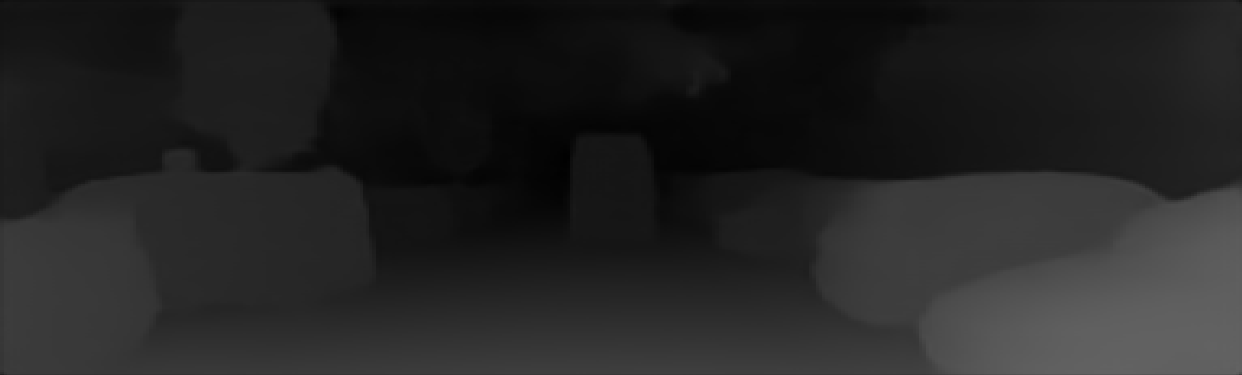
\includegraphics[width=3in]{figures/cmp_kitti/pred_029}}
		\vspace{-10pt}
		\centerline{DispNetC}
	\end{minipage}
	\vfill
	%----------------------第2行----------------------
	\begin{minipage}{0.48\linewidth}
		\centerline{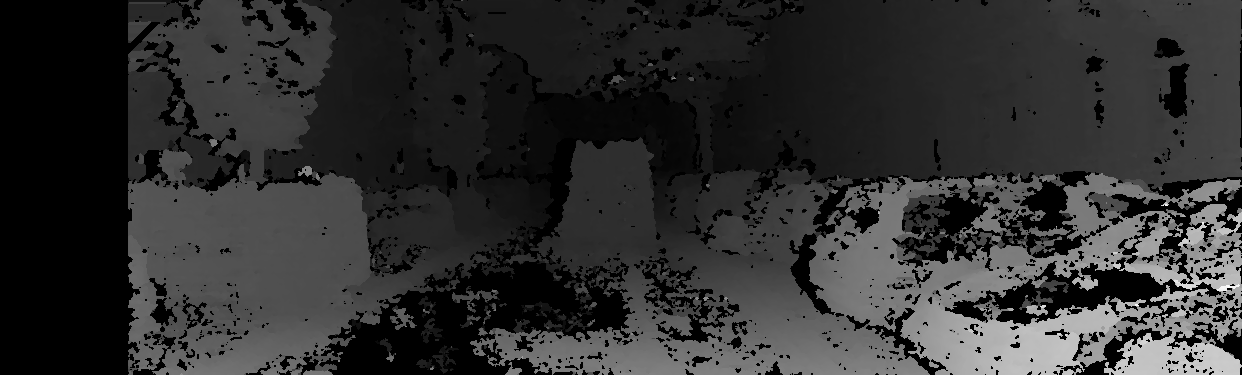
\includegraphics[width=3in]{figures/cmp_kitti/sgm_029}}
		\vspace{-10pt}
		\centerline{SGM}
	\end{minipage}
	\hfill
	\begin{minipage}{0.48\linewidth}
		\centerline{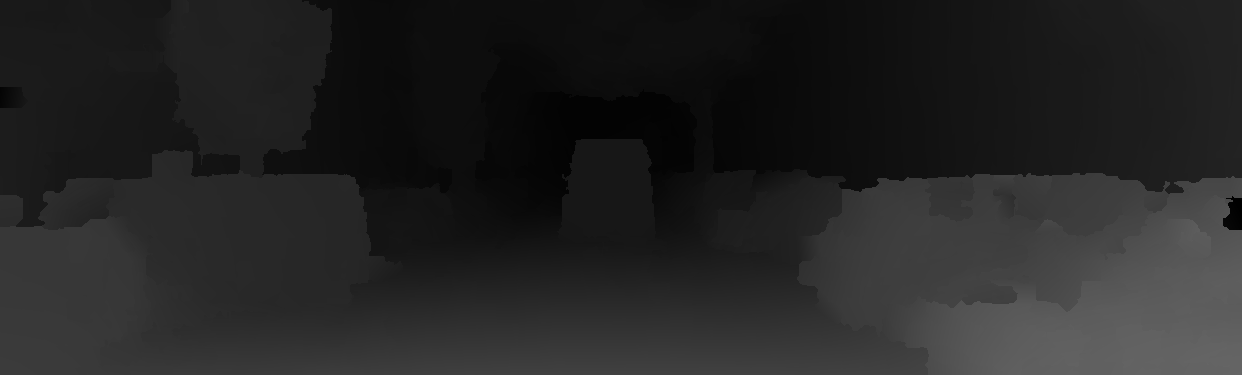
\includegraphics[width=3in]{figures/cmp_kitti/sps_029}}
		\vspace{-10pt}
		\centerline{SPS-St}
	\end{minipage}
	%<<<<<<<<<<<<<<<<<<<<第1组<<<<<<<<<<<<<<<<<<<<
	%>>>>>>>>>>>>>>>>>>>>第2组>>>>>>>>>>>>>>>>>>>>
	%----------------------第1行-----------------------
	\begin{minipage}{0.48\linewidth}
		\centerline{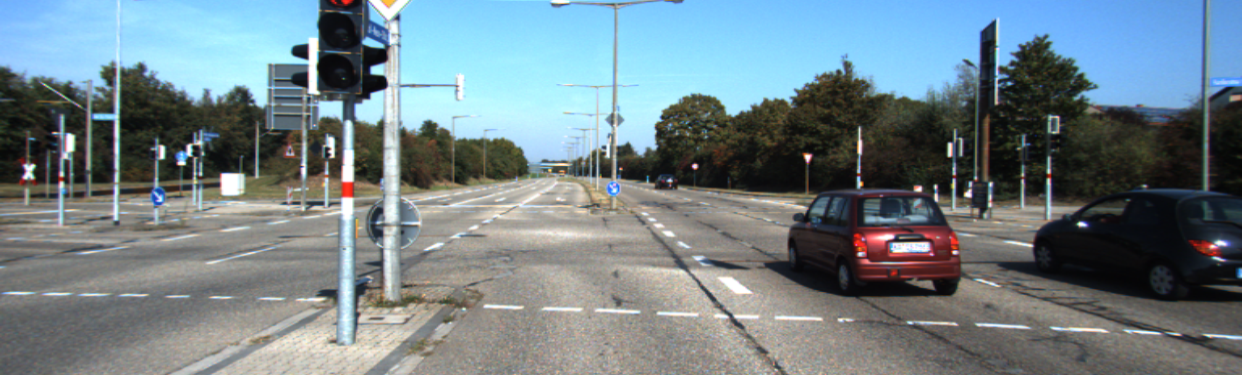
\includegraphics[width=3in]{figures/cmp_kitti/l_031}}
		\vspace{-10pt}
		\centerline{左图}
	\end{minipage}
	\hfill
	\begin{minipage}{0.48\linewidth}
		\centerline{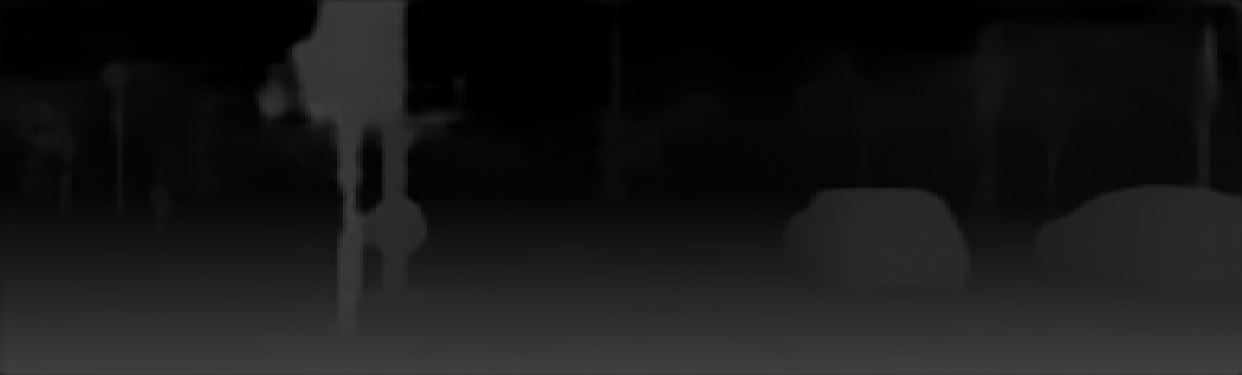
\includegraphics[width=3in]{figures/cmp_kitti/pred_031}}
		\vspace{-10pt}
		\centerline{DispNetC}
	\end{minipage}
	\vfill
	%----------------------第2行----------------------
	\begin{minipage}{0.48\linewidth}
		\centerline{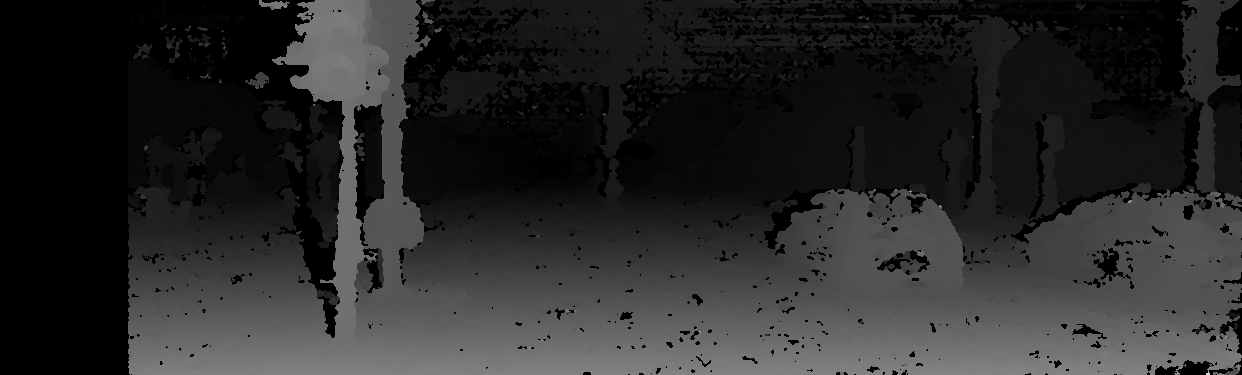
\includegraphics[width=3in]{figures/cmp_kitti/sgm_031}}
		\vspace{-10pt}
		\centerline{SGM}
	\end{minipage}
	\hfill
	\begin{minipage}{0.48\linewidth}
		\centerline{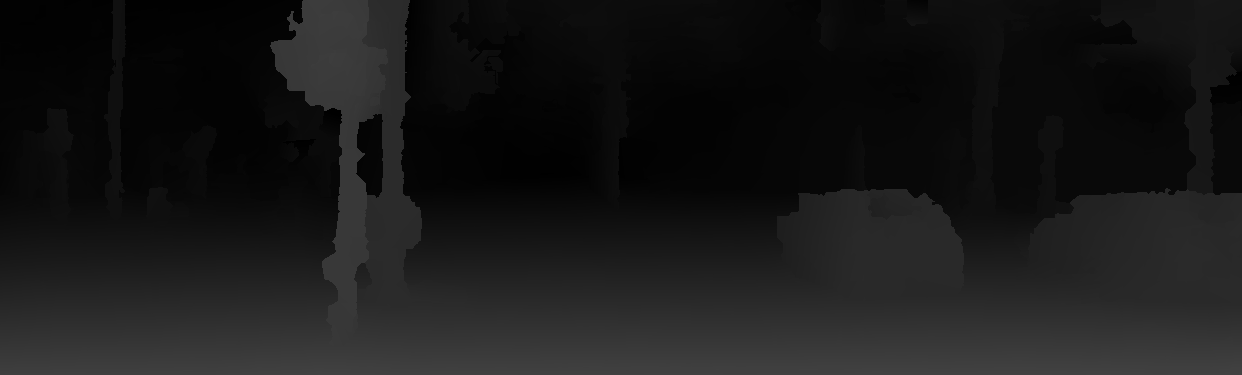
\includegraphics[width=3in]{figures/cmp_kitti/sps_031}}
		\vspace{-10pt}
		\centerline{SPS-St}
	\end{minipage}
	%<<<<<<<<<<<<<<<<<<<<第2组<<<<<<<<<<<<<<<<<<<<
	%>>>>>>>>>>>>>>>>>>>>第3组>>>>>>>>>>>>>>>>>>>>
	%----------------------第1行-----------------------
	\begin{minipage}{0.48\linewidth}
		\centerline{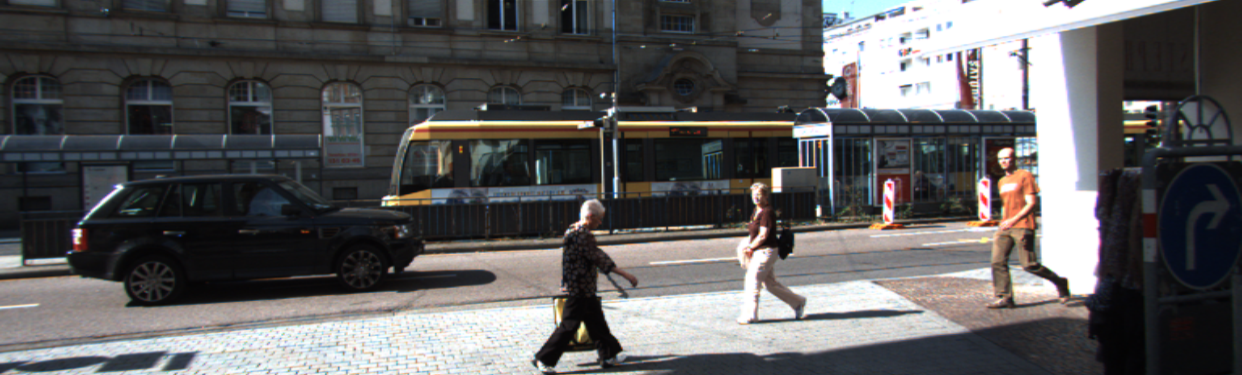
\includegraphics[width=3in]{figures/cmp_kitti/l_032}}
		\vspace{-10pt}
		\centerline{左图}
	\end{minipage}
	\hfill
	\begin{minipage}{0.48\linewidth}
		\centerline{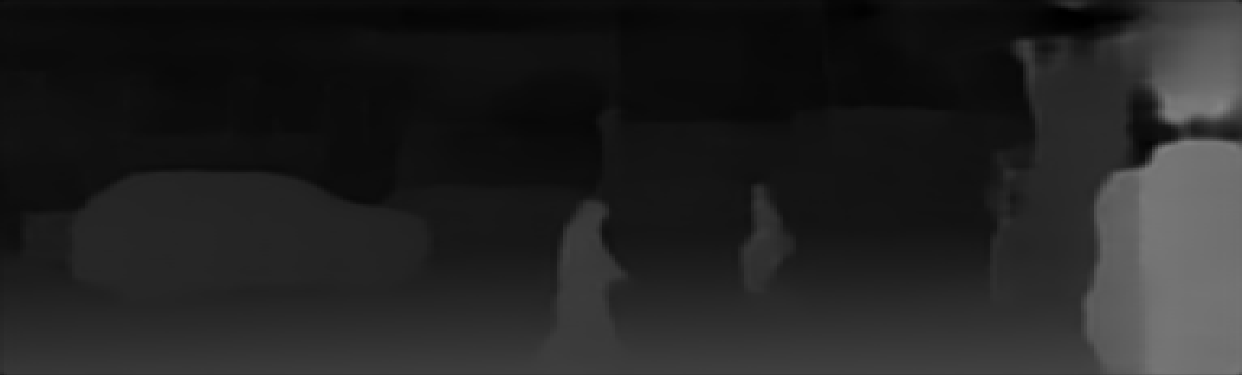
\includegraphics[width=3in]{figures/cmp_kitti/pred_032}}
		\vspace{-10pt}
		\centerline{DispNetC}
	\end{minipage}
	\vfill
	%----------------------第2行----------------------
	\begin{minipage}{0.48\linewidth}
		\centerline{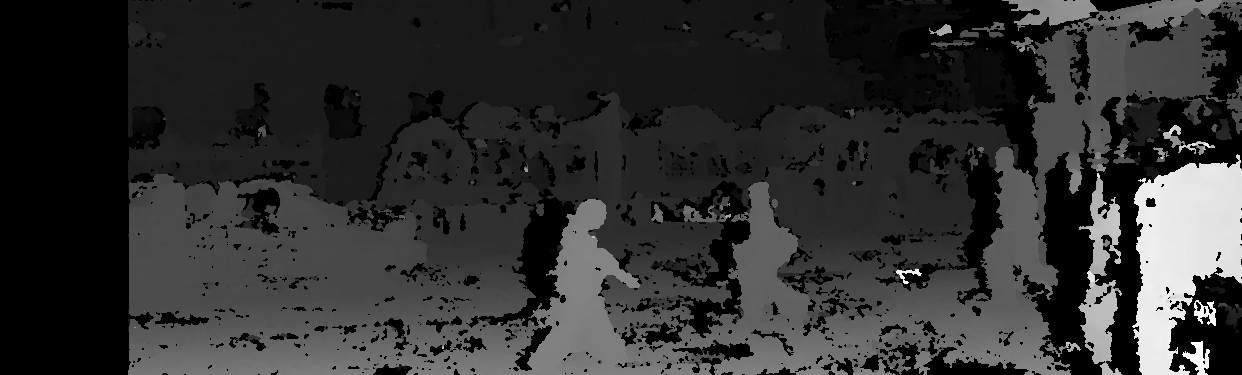
\includegraphics[width=3in]{figures/cmp_kitti/sgm_032}}
		\vspace{-10pt}
		\centerline{SGM}
	\end{minipage}
	\hfill
	\begin{minipage}{0.48\linewidth}
		\centerline{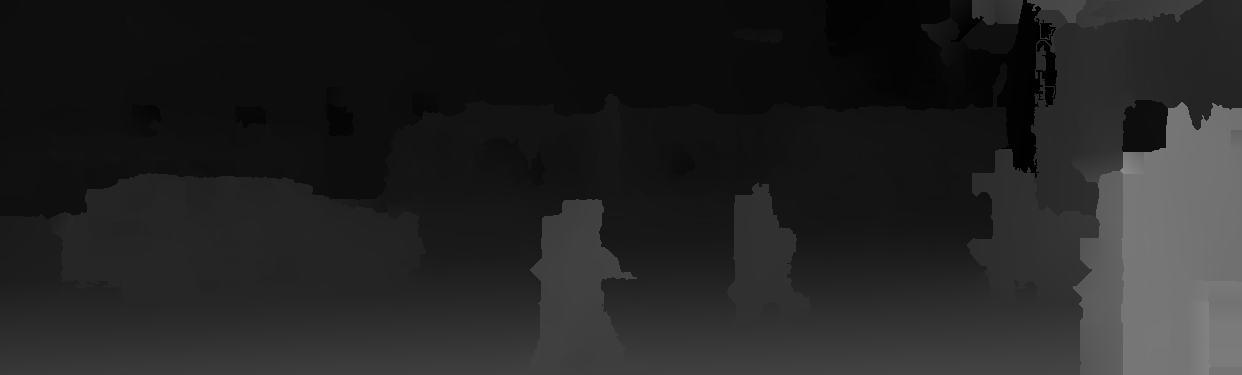
\includegraphics[width=3in]{figures/cmp_kitti/sps_032}}
		\vspace{-10pt}
		\centerline{SPS-St}
	\end{minipage}
	%<<<<<<<<<<<<<<<<<<<<第3组<<<<<<<<<<<<<<<<<<<<
	%>>>>>>>>>>>>>>>>>>>>第4组>>>>>>>>>>>>>>>>>>>>
%----------------------第1行-----------------------
\begin{minipage}{0.48\linewidth}
	\centerline{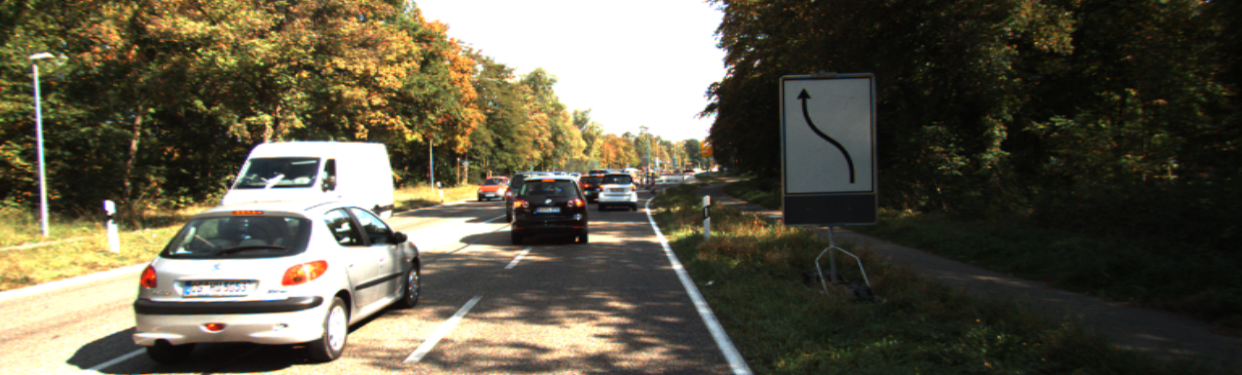
\includegraphics[width=3in]{figures/cmp_kitti/l_097}}
	\vspace{-10pt}
	\centerline{左图}
\end{minipage}
\hfill
\begin{minipage}{0.48\linewidth}
	\centerline{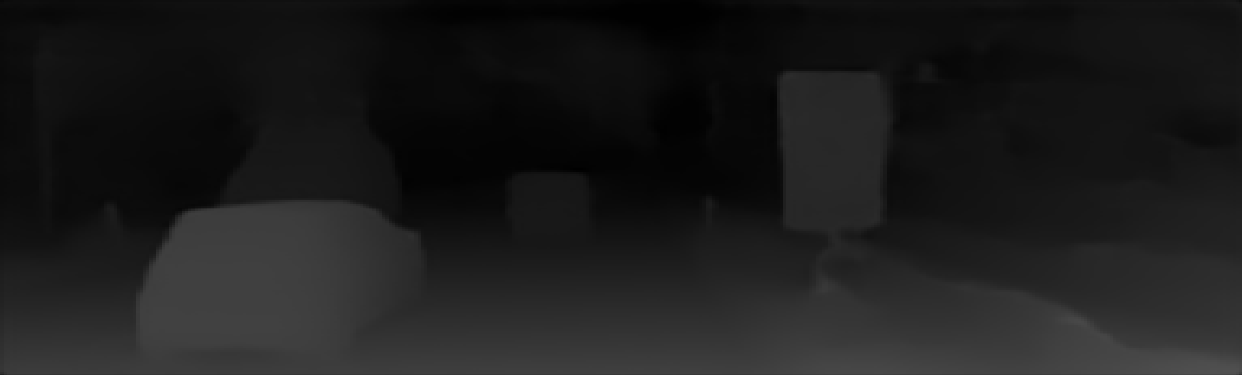
\includegraphics[width=3in]{figures/cmp_kitti/pred_097}}
	\vspace{-10pt}
	\centerline{DispNetC}
\end{minipage}
\vfill
%----------------------第2行----------------------
\begin{minipage}{0.48\linewidth}
	\centerline{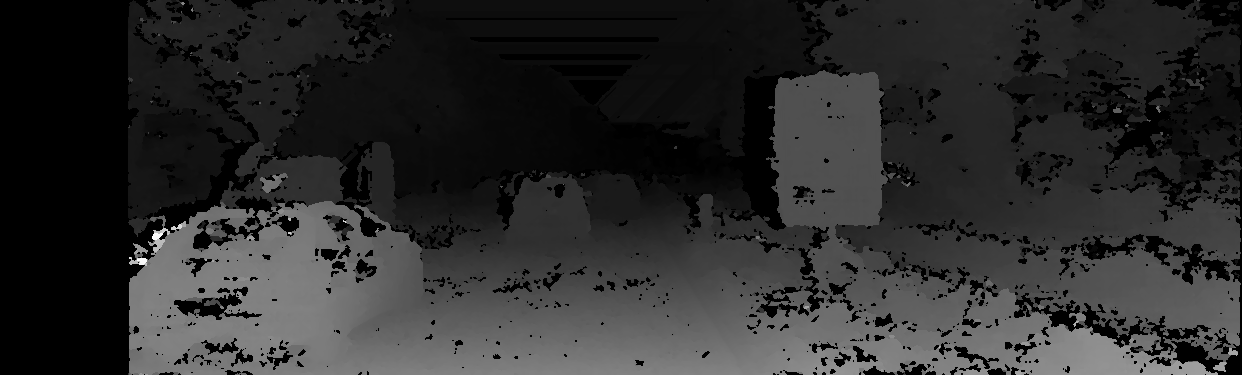
\includegraphics[width=3in]{figures/cmp_kitti/sgm_097}}
	\vspace{-10pt}
	\centerline{SGM}
\end{minipage}
\hfill
\begin{minipage}{0.48\linewidth}
	\centerline{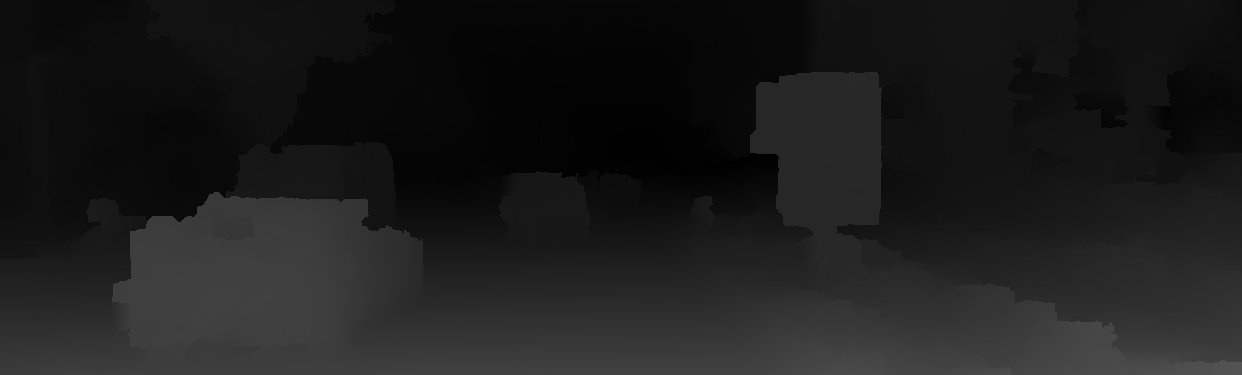
\includegraphics[width=3in]{figures/cmp_kitti/sps_097}}
	\vspace{-10pt}
	\centerline{SPS-St}
\end{minipage}
%<<<<<<<<<<<<<<<<<<<<第4组<<<<<<<<<<<<<<<<<<<<
	\caption{DispNetC, SGM和SPS-St在KITTI2015部分图片上的测试结果}
\label{fig:4_3_kitti_cmp_result}
\end{figure}

%三种算法在KITTI2015数据集上的误差对比
\begin{table}[!htb]
	\centering
	\caption{不同匹配算法在KITTI2015数据集上的对比}
	\label{tab:4_3_cmp_kitti}
%	\begin{small} %{scriptsize}
		\begin{tabular}{|c|c|c|c|}\hline
			方法          & 平均视差误差(px) & 平均错误率(\%) & 运行时间(s) \\\hline
			%---------------------------------------------------------
			AD            & 11.56                      & 32.02                 & --      \\
			CCNN      & 8.50                       & 17.70                  & --      \\
			OCV-BM &  --                           & 25.27                  &  0.1    \\
			SGM         & --                            & 10.86                 &  1.1     \\
			SPS-St    & --                            & 5.31                    & 2         \\
			DispNetC & 1.37                       & 7.74                   & \textbf{0.06}  \\\hline
		\end{tabular}
%	\end{small} %{scriptsize}
\end{table}


\subsubsection{训练集大小对实验结果的影响}
为了研究训练集大小对实验结果的影响,在微调时分别使用KITTI2015训练数据的20\%、40\%、60\%、80\%(即40、80、120和160组图片)对网络进行训练,在剩余40组图片上进行验证,实验结果见图\ref{fig:4_3_kitti_dataset_size}和表\ref{tab:4_3_kitti_dataset_size}。

%训练集大小对实验结果的影响
\begin{table}[!htb]
	\centering
	\caption{训练集大小对实验结果的影响}
	\label{tab:4_3_kitti_dataset_size}
%	\begin{small}
		\begin{tabular}{|c|c|c|c|}\hline
			训练数据量 & 平均视差误差(px) & 平均错误率(\%) \\\hline
			%---------------------------------------------------------
			40               & 1.9126                   & 11.94                  \\
			80               & 1.7924                   & 9.60                   \\
			120             & 1.4898                  & 9.23                    \\
			160             & 1.3746                  & 7.74                    \\\hline
		\end{tabular}
%	\end{small}
\end{table}

\vspace{1in}

% 不同训练集大小下的测试误差变化趋势
\begin{figure}[!htb]
	\centering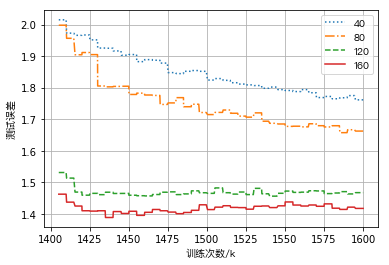
\includegraphics[width=4in]{figures/4_3_kitti_dataset_size}
	\caption{不同训练集大小下的测试误差变化趋势}\label{fig:4_3_kitti_dataset_size}
\end{figure}


由表中结果可以得知,训练数据集越大,训练出的网络模型就越好,最终网络的匹配精度就越高。因此,使用更多的真实训练数据是提高匹配准确度的最直接的方法。

%TODO: 网络结构的参数选择/数据增强/光照变化对结果的影响。

%------------------------------------------------------------------------------------
\section{本章小结}
本章主要介绍了基于卷积神经网络模型DispNetC的立体匹配。首先简要梳理了传统立体匹配算法,然后详细地介绍了网络基础架构DispNet和加入相关层得到的DispNetC的网络结构,包括收缩部分和扩张部分各网络层的具体参数。接下来阐述了网络的训练方法和相关训练参数设置,之后在FlyingThings3D和KITTI2015数据集上对网络进行了训练和微调,给出了训练完成后的测试结果,并与SGM、SPS-St等算法进行了对比。测试结果表明DispNetC网络模型的匹配精度较高,且运行速度很快,适合应用于旋翼无人机等对实时性要求较高的场景。最后讨论了训练集大小对网络匹配精度的影响,比较结果说明增大训练数据量有利于提高匹配精度。







